\باب{مرتعش} \شناخت{باب_مرتعش}
گزشتہ باب میں \اصطلاح{منفی واپسی ادوار} پر غور کیا گیا۔اس باب میں \اصطلاح{مرتعش}\حاشیہب{oscillator} پر غور کیا جائے گا جو \اصطلاح{مثبت واپسی دور} کی ایک قسم ہے۔\اصطلاح{مرتعش} ایک ایسے دور کو کہتے ہیں جسے کوئی داخلی اشارہ دئے بغیر اس سے ارتعاش کرتا خارجی اشارہ حاصل کیا جاتا ہے۔آئیں مرتعش کی بنیادی کارکردگی شکل \حوالہ{شکل_بنیادی_مثبت_واپسی_دور} کی مدد سے سمجھیں۔ 
\begin{figure}
\centering

\includegraphics[scale=0.90]{feedbackBasicPositive}
\caption{مثبت واپسی دور}
\label{شکل_بنیادی_مثبت_واپسی_دور}
\end{figure}
تصور کریں کہ ایک لمحے کے لئے اس دور کو ارتعاش کرتا داخلی اشارہ \عددیء{X_s} فراہم کرنے کے بعد \عددیء{X_s=0} کر دیا جاتا ہے۔اس طرح ایک لمحے کے لئے اس دور میں  ارتعاش کرتا خارجی اشارہ \عددیء{X_o} نمودار ہو  گا۔واپسی دور \عددیء{X_o} سے \عددیء{X_f=WX_o} پیدا کرے گا جو کہ بنیادی ایمپلیفائر کو بطور داخلی اشارہ مہیا کیا گیا ہے۔بنیادی ایمپلیفائر \عددیء{X_f} سے خارجی اشارہ \عددیء{X_o=AX_f=WAX_o} پیدا کرے گا۔یوں واپسی دور اور بنیادی ایمپلیفائر میں ایک چکر کے بعد پہلی مرتبہ نمودار ہونے والے اشارے \عددیء{X_o} کی قیمت اب \عددیء{WAX_o} ہو گی۔یہ اشارہ بھی جب واپسی دور اور بنیادی ایمپلیفائر میں ایک چکر کاٹے تو اس کی نئی قیمت \عددیء{(WA)^2 X_o} ہو جائے گی۔اسی طرح \عددیء{n} چکر کے بعد بنیادی ایمپلیفائر کا خارجی اشارہ \عددیء{(WA)^n X_o} ہو گا۔اب اگر \عددیء{WA=1} ہو تب \عددیء{n} چکر کے بعد بھی بنیادی ایمپلیفائر کا خارجی اشارہ \عددیء{1^n X_o = X_o} ہی ہو گا۔اس طرح اگرچہ اس دور کو کوئی داخلی اشارہ نہیں دیا جا رہا یہ پھر بھی ارتعاش کرتا اشارہ \عددیء{X_o} خارج کرتا رہے گا۔ایسی خوبی رکھنے والے دور کو \اصطلاح{مرتعش}  کہتے ہیں۔

اس کے برعکس اگر \عددیء{WA} کی قیمت ایک (1) سے کم ہو، مثلاً \عددیء{WA=0.9} ہو، تب پہلی مرتبہ نمودار ہونے والا اشارہ \عددیء{X_o} ایک چکر کے بعد کم ہو کر \عددیء{0.9 X_o} رہ جائے گا۔دو چکر کے بعد اس کی قیمت مزید کم ہو کر \عددیء{(0.9)^2 X_o =0.81 X_o} رہ جائے گی اور یوں ہر چکر کے بعد بنیادی ایمپلیفائر کا خارجی اشارہ کم ہوتے ہوتے آخر کار صفر قیمت اختیار کر لے گا۔

اسی طرح  اگر  \عددیء{WA} کی قیمت ایک (1) سے زیادہ ہو، مثلاً \عددیء{WA=1.1} ہو، تب پہلی مرتبہ نمودار ہونے والا اشارہ \عددیء{X_o} ایک چکر کے بعد بڑھ کر \عددیء{1.1 X_o} ہو جائے گا۔دو چکر کے بعد اس کی قیمت مزید بڑھ کر \عددیء{(1.1)^2 X_o =1.21 X_o} ہو جائے گی اور یوں ہر چکر کے بعد بنیادی ایمپلیفائر کا خارجی اشارہ بڑھتا رہے گا۔خارجی اشارہ بڑھتے بڑھتے اس مقام تک پہنچ جائے گا جہاں بنیادی ایمپلیفائر غیر خطی خطے میں داخل ہونا شروع ہو جائے گا۔ غیر خطی خطے میں داخل ہوتے ہوئے بنیادی ایمپلیفائر کے افزائش کی قیمت گھٹنا شروع ہو جائے گی اور یوں خارجی اشارے کے حیطے کا بڑھنا پہلے کم اور آخر کار اس کا بڑھنا مکمل طور   رک  جائے  گا۔ جہاں ٹرانزسٹر کی افزائش سے اشارے کا حیطہ بڑھنا اور اشارے کا حیطہ بڑھنے سے ٹرانزسٹر کی افزائش کم ہونے کے اعمال توازن اختیار کر لیں، وہیں ارتعاشی اشارے کا حیطہ برقرار رہتا ہے۔یہ اعمال غیر خطی نوعیت کے ہوتے ہیں جنہیں قلم و کاغذ سے حل کرتے ہوئے مرتعش کے خارجی اشارے کے حیطے کا حساب لگانا نہایت مشکل ہوتا ہے۔

کسی بھی مرتعش میں زیادہ دیر  \عددیء{WA=1} رکھنا ممکن نہیں ہوتا۔درجہ حرارت میں تبدیلی، وقت کے ساتھ برقیاتی پرزہ جات میں تبدیلی اور ایسے دیگر  وجوہات کی بنا پر مرتعش چالو کرتے ہی \عددیء{WA \ne 1} ہو جائے گا۔اگر  \عددیء{WA < 1} ہو جائے تو ایسی صورت میں مرتعش رکھ جائے گا۔اس کے برعکس اگر \عددیء{WA} کی قیمت  \عددیء{1} سے قدرِ زیادہ ہو جائے تو ایسی صورت میں مرتعش برقرار ارتعاشی اشارہ خارج کرتا ہے۔

مرتعش کے اس بنیادی اصول جسے مساوت \حوالہ{مساوات_برکہازن_کا_اصول} میں دوبارہ دکھایا گیا ہے کو \اصطلاح{برکہازن کا اصول}\فرہنگ{برکہازن کا اصول}\فرہنگ{Barkhausen criteria}\حاشیہب{Barkhausen criteria} کہتے ہیں۔\حاشیہد{جرمنی کے عالم طبیعیات ہائنرچ  برکہازن نے اس اصول کو پیش کیا}
\begin{align} \label{مساوات_برکہازن_کا_اصول}
WA =1
\end{align}
اس مساوات کے دو پہلو ہیں۔اس مساوات کے تحت \عددیء{\abs{WA}=1} اور ساتھ ہی ساتھ \عددیء{\phase {WA}=2 m \pi} ہونا ضروری ہے جہاں \عددیء{m=0,1,2 \cdots}  ہو سکتا ہے۔یوں اسے یوں لکھنا زیادہ بہتر ہے۔
\begin{align} \label{مساوات_برکہازن_کا_اصول_الف}
\abs{WA} &=\num{1}\\
\phase{WA} &=2m \pi 
\end{align}
آپ دیکھ سکتے ہیں کہ حقیقت میں کسی بھی مرتعش کو برقرار کام کرتے رکھنے کے لئے یہ ضروری ہے کہ \عددیء{\abs{WA} >1}  رکھا جائے۔حقیقت میں
 \عددیء{ \abs{WA} > 1.05} رکھا جاتا ہے۔
 
مندرجہ بالا تذکرے میں تصور کیا گیا کہ مرتعش کو چالو کرنے کی خاطر ایک لمحے کے لئے \عددیء{X_s} فراہم کیا گیا۔ حقیقت میں مرتعش کو چالو کرتے وقت اسے عموماً کسی قسم کا ارتعاش کرتا اشارہ نہیں مہیا کیا جاتا۔کسی بھی دور جسے برقی طاقت مہیا نہیں کیا گیا ہو غیر چالو رہتا ہے اور ایسی صورت  میں اس کے تمام اشارات صفر وولٹ (صفر ایمپیئر) ہوتے ہیں۔اس طرح جب مرتعش کو برقی طاقت مہیا کر کے غیر چالو حالت سے چالو کیا جائے تو اس کے مختلف حصے چند ہی لمحوں میں غیر چالو صورت سے یک سمتی  مائل کردہ  صورت اختیار کر لیتے ہیں۔یوں ان لمحات کے دوران مرتعش پر پائے جانے والے تمام اشارات تغیر پذیر ہوتے ہیں جنہیں ہم چالو کرتے وقت کی برقی شور تصور کر سکتے ہیں۔مرتعش عموماً اسی برقی شور سے چالو ہو کر ارتعاش پذیر ہوتا ہے۔البتہ اگر کہیں ایسی صورت پائی جائے کہ مرتعش چالو ہوتے وقت ازخود ارتعاش پذیر نہیں ہو پاتا ہو یا اگر برقی شور کا سہارا لیتے ہوئے مرتعش کو چالو کرنا قابل قبول نہ ہو تب مرتعش کو چالو کرنے کی خاطر بیرونی اشارہ چند لمحات کے لئے مہیا کیا جاتا ہے۔\حاشیہد{مجھے گزشتہ پچیس سالوں میں صرف ایک مرتبہ مرتعش کو چالو کرنے کی خاطر اشارہ مہیا کرنا پڑا ہے۔} 

اب تک کی گفتگو میں خارجی اشارے کی شکل پر کسی قسم کی بحث نہیں کی گئی۔حقیقت میں مرتعش کے خارجی اشارے کی شکل کچھ بھی ہو سکتی ہے البتہ اس باب میں صرف سائن نما خارجی اشارہ پیدا کرنے والے مرتعش پر غور کیا جائے گا جن میں ٹرانزسٹر ایمپلیفائر  استعمال کرتے ہوئے واپسی اشارے کو مزاحمت، کپیسٹر، امالہ، ٹرانسفارمر وغیرہ کی مدد سے حاصل کیا جاتا ہے۔

واپسی دور میں کپیسٹر اور امالہ (یعنی برقی رکاوٹ) کے استعمال سے واپس کار کے مستقل کی قیمت از خود تعدد \عددیء{\omega} پر منحصر ہوتی ہے۔یوں اس کو \عددیء{W(\omega)} لکھنا زیادہ درست ہو گا۔ایسی صورت میں \اصطلاح{برکہازن کا اصول}  \عددیء{\abs{W(\omega) A}=1}  عموماً کسی ایک ہی تعدد پر پورا  اترے گا۔آپ جانتے ہیں کہ کسی بھی غیر سائن نما لہر کو \اصطلاح{فوریئر تسلسل}\حاشیہب{fourier series} کی مدد سے لکھا جا سکتا ہے۔فوریئر تسلسل میں \عددیء{\omega_o}، \عددیء{2 \omega_o}، \عددیء{3 \omega_o}، \عددیء{\نقطے} تعدد پر لامحدود اجزاء پائے جاتے ہیں۔چالو کرتے وقت کے برقی شور کی بھی فوریئر تسلسل لکھی جا سکتی ہے جہاں سے صاف ظاہر ہے کہ اس میں بھی تمام تعدد پائے جاتے ہیں۔مرتعش ان میں سے صرف اس تعدد پر ارتعاش کرے گا جو \اصطلاح{برکہازن کے اصول} پر پورا اترتا ہو۔

\حصہ{مرتعش کی تخلیق}
شکل \حوالہ{شکل_مرتعش_کی_تخلیق} الف میں بنیادی ایمپلیفائر دکھایا گیا ہے۔اس کے خارجی اشارے \عددیء{V_o} اور داخلی اشارے \عددیء{V_i} کے مابین \عددیء{\SI{180}{\degree}} کا زاویہ ہے۔اگر اسے استعمال کرتے ہوئے مرتعش تخلیق دینا ہو تو واپس کار کو مزید \عددیء{\SI{180}{\degree}} کا زاویہ پیدا کرنا ہو گا۔
\begin{figure}
\centering
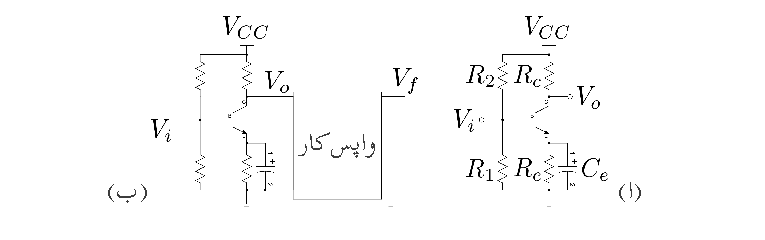
\includegraphics[scale=0.90]{basicRCoscillatorAmplifier}
\caption{مرتعش کی تخلیق}
\label{شکل_مرتعش_کی_تخلیق}
\end{figure}
شکل  ب میں واپس کار کو ڈبے کی شکل میں دکھایا گیا ہے۔یوں \عددیء{V_f} اور \عددیء{V_o} کے درمیان \عددیء{\SI{180}{\degree}} کا زاویہ درکار ہے۔ٹرانزسٹر کو \عددیء{V_f}  بطور داخلی اشارہ مہیا کرنے سے مرتعش حاصل ہوتا ہے۔مندرجہ ذیل مثال میں اشارات کے مابین زاویہ پیدا کرنے کا ایک طریقہ دکھایا گیا ہے۔
%==================
\ابتدا{مثال}
شکل \حوالہ{شکل_مزاحمت_کپیسٹر_زاویہ_میں_تبدیلی} الف میں \عددیء{\hat{V_o}} اور \عددیء{\hat{V_i}} کے درمیان زاویہ کی مساوات حاصل کریں۔
\begin{itemize}
\item
\عددیء{\SI{10}{\kilo \hertz}} پر \عددیء{C=\SI{0.1}{\micro \farad}}اور \عددیء{R=\SI{1}{\kilo \ohm}} لیتے ہوئے اس زاویہ کی قیمت حاصل کریں۔
\item
مزاحمت \عددیء{R} کی وہ قیمت حاصل کریں جس پر یہ زاویہ \عددیء{\SI{-60}{\degree}} ہو گا۔
\end{itemize}
%
\begin{figure}
\centering
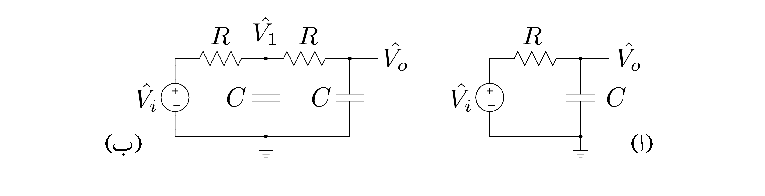
\includegraphics[scale=0.90]{RCphaseShiftExample}
\caption{مزاحمت-کپیسٹر کی مدد سے اشارات کے زاویہ میں تبدیلی}
\label{شکل_مزاحمت_کپیسٹر_زاویہ_میں_تبدیلی}
\end{figure}

حل:
\عددیء{\hat{V_i} = V \phase{\SI{0}{\degree}}} لیتے ہوئے، دائرے میں برقی رو \عددیء{\hat{I}} لکھتے ہوئے کرخوف کے قانون برائے برقی دباو سے حاصل ہوتا ہے
\begin{align*}
\hat{I}=\frac{V \phase{\SI{0}{\degree}}}{R+\frac{1}{j\omega C}}
\end{align*}
اور یوں
\begin{align*}
\hat{V_0}= \hat{I} \times \left(\frac{1}{j\omega C} \right)&=\frac{V\phase{0}}{1+j \omega R C}\\
&=\frac{V}{\sqrt{1+R^2 \omega^2 C^2}} \phase{-\tan^{-1} \left(\omega R C \right)}
\end{align*}
جس سے داخلی اور خارجی اشارات کے مابین زاویہ
\begin{align*}
\phase{\theta}=-\tan^{-1} \left(\omega R C \right) 
\end{align*}
حاصل ہوتا ہے۔یوں
\begin{itemize}
\item
$\phase{\theta}=-\tan^{-1} \left(-2 \times \pi \times 10000\times 1000 \times 0.1 \times 10^{-6} \right)=\SI{-81}{\degree} $
\item
\begin{align*}
-\tan^{-1}\left(2 \times \pi \times 10000 \times R \times 0.1 \times 10^{-6}\right)=\SI{-60}{\degree}\\
R=\SI{276}{\ohm}
\end{align*}
\end{itemize}
حاصل ہوتے ہیں۔
\انتہا{مثال}

مندرجہ بالا مثال کو دیکھتے ہوئے ایسا معلوم ہوتا ہے کہ مزاحمت-کپیسٹر کے دو کڑیاں استعمال کرتے ہوئے دگنا زاویہ حاصل کیا جا سکتا ہے۔یہ بات درست ثابت ہوتی ہے، البتہ جیسے آپ سوال \حوالہ{سوال_مرتعش_مزاحمت_کپیسٹر_دو_کڑی} میں دیکھیں گے، دو کڑی \عددیء{RC} کا زاویہ حاصل کرتے وقت نسبتاً لمبی مساوات حل کرنی ہو گی۔

\عددیء{R} اور \عددیء{C} کے ضرب \عددیء{RC} کو بڑھا کر زیادہ زاویہ حاصل کیا جاتا ہے۔لامحدود \عددیء{RC} یعنی\عددیء{RC = \infty} پر \عددیء{\SI{90}{\degree}} حاصل ہوتا ہے۔حقیقت میں لامحدود \عددیء{RC} استعمال کرنا ممکن نہیں ہوتا لہٰذا ایک عدد مزاحمت اور ایک عدد کپیسٹر استعمال کرتے ہوئے \عددیء{\SI{90}{\degree}} حاصل کرنا ممکن نہیں ہوتا۔یوں \عددیء{RC} کے دو کڑیوں سے \عددیء{\SI{180}{\degree}} حاصل نہیں کیا جا سکتا۔حقیقت میں کم از کم تین \عددیء{RC} کڑیاں استعمال کرتے ہوئے \عددیء{\SI{180}{\degree}} حاصل کیا جاتا ہے۔مندرجہ ذیل حصے میں مزاحمت-کپیسٹر مرتعش میں ایسا ہی کیا گیا ہے۔  


\حصہ{مزاحمت-کپیسٹر \عددیء{RC} مرتعش}
شکل \حوالہ{شکل_مزاحمت_کپیسٹر_مرتعش} الف میں ٹرانزسٹر ایمپلیفائر پر مبنی مرتعش دکھایا گیا ہے جس میں کلکٹر پر پائے جانے والے اشارے \عددیء{X_0} سے واپس کار  \عددیء{X_f} پیدا کرتا ہے۔ٹرانزسٹر اپنے  بیس پر پائے جانے والے اشارے کے حیطے کو بڑھا کر جبکہ اس کے زاویہ میں \عددیء{\SI{180}{\degree}}  کے تبدیلی کے ساتھ اسے کلکٹر پر خارج کرتا ہے۔یوں بنیادی ایمپلیفائر اور واپس کار کے دائرے میں ایک چکر کے بعد کل زاویہ میں تبدیلی کو \عددیء{\SI{0}{\degree}} رکھنے کی خاطر واپس کار کو بھی \عددیء{\SI{180}{\degree}} کی تبدیلی پیدا کرنا ہو گی۔جیسا اوپر مثال میں دکھایا گیا، مزاحمت-کپیسٹر \عددیء{RC} کے کڑیاں استعمال کرتے ہوئے ایسا کرنا ممکن ہے۔شکل \حوالہ{شکل_مزاحمت_کپیسٹر_مرتعش} الف میں مزاحمت اور کپیسٹر کو  شکل \حوالہ{شکل_مزاحمت_کپیسٹر_زاویہ_میں_تبدیلی} الف سے قدر مختلف طرز پر جوڑا گیا ہے۔ 

بنیادی ایمپلیفائر \عددیء{Q}، \عددیء{R_1}، \عددیء{R_2}، \عددیء{R_c}، \عددیء{R_e} اور \عددیء{C_e} پر مشتمل ہے۔ مرتعش کے خارجی تعدد پر کپیسٹر \عددیء{C_e} بطور قصر دور کام کرتا ہے۔بنیادی ایمپلیفائر میں واپس کار شامل کرنے سے مرتعش حاصل ہوتا ہے۔واپس کار تین عدد کپیسٹر اور تین عدد مزاحمت سے حاصل کیا گیا ہے۔شکل  ب میں ٹرانزسٹر کا پائے \عددیء{\pi} ریاضی نمونہ استعمال کرتے ہوئے اس مرتعش کا مساوی دور دکھایا گیا ہے جس میں \عددیء{R_e} کو قصر دو کیا گیا ہے۔جیسے آپ دیکھ سکتے ہیں \عددیء{r_{be}}، \عددیء{R_1} اور \عددیء{R_2} متوازی جڑے ہیں۔ ان متوازی جڑے مزاحمت کی کل قیمت کو \عددیء{R_m} لکھا گیا ہے۔یوں \عددیء{R_m} اور \عددیء{R'} سلسلہ وار جڑے ہیں- حقیقت میں \عددیء{r_{be}} کی قیمت \عددیء{R_1} اور \عددیء{R_2} کے قیمتوں سے نہایت کم ہوتی ہے اور یوں \عددیء{R_m} کی قیمت تقریباً \عددیء{r_{be}} کے ہی برابر ہوتی ہے یعنی \عددیء{R_m \approx r_{be}} ہوتا ہے۔اگر \عددیء{R'} کی قیمت یوں منتخب کی جائے کہ \عددیء{R'+R_m=R} ہو تب ہم دیکھتے ہیں کہ واپسی دور تین یکساں  \عددیء{RC} حصوں پر مشتمل ہوتا ہے۔اگرچہ واپسی دور کے تین کپیسٹروں کی قیمت آپس میں برابر یا تین مزاحمتوں کی قیمت آپس میں برابر رکھنا لازم نہیں، البتہ ایسا رکھنے سے مرتعش پر ترسیلی غور نسبتاً آسان ہو جاتا ہے۔ہم ایسا ہی کرتے ہیں۔
\begin{figure}
\centering
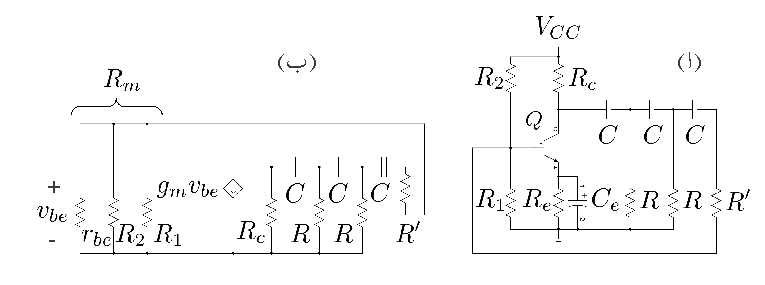
\includegraphics[scale=0.90]{phaseShiftOscillator}
\caption{مزاحمت-کپیسٹر مرتعش یا \عددیء{RC} مرتعش}
\label{شکل_مزاحمت_کپیسٹر_مرتعش}
\end{figure}
شکل \حوالہ{شکل_مزاحمت_کپیسٹر_مرتعش_الف} پر نظر رکھیں جہاں \عددیء{R_m \approx r_{be}} لیا گیا ہے اور \عددیء{R'+r_{be}} کو \عددیء{R} کے برابر رکھا گیا ہے۔یوں
\begin{align*}
V_1 &=I_0 \left(R+\frac{1}{j \omega C} \right)
\end{align*}
ہو گا جسے استعمال کرتے ہوئے ہم لکھ سکتے ہیں
\begin{align*}
I_1 &=\frac{V_1}{R}=I_0 \left (1+\frac{1}{j \omega C R} \right)
\end{align*}
اس طرح
\begin{align*}
I_2 =I_1+I_0=I_0 \left (2+\frac{1}{j \omega C R} \right)
\end{align*}
ہو گا۔ چونکہ \عددیء{V_2 - V_1 =\frac{I_2}{j \omega C}} کے برابر ہے لہٰذا
\begin{align*}
V_2 &=V_1+\frac{I_2}{j \omega C} \\
&=I_0 \left (R+\frac{1}{j \omega C} \right )+\frac{I_0}{j \omega C} \left (2+\frac{1}{j \omega C R} \right )\\
&=I_0 \left [R+\frac{3}{j \omega C} +\frac{1}{\left(j \omega C \right )^2 R}\right ]
\end{align*}
یوں
\begin{align*}
I_3=\frac{V_2}{R}=I_0 \left [1+\frac{3}{j \omega C R}+\frac{1}{\left(j \omega C R \right )^2} \right ]
\end{align*}
اور
\begin{align*}
I_4 &=I_3 +I_2\\
&=I_0 \left [1+\frac{3}{j \omega C R}+\frac{1}{\left(j \omega C R \right )^2} \right ]+I_0 \left [2+\frac{1}{j \omega C R} \right] \\
&=I_0 \left[3+\frac{4}{j \omega C R}+\frac{1}{\left (j \omega C R \right )^2} \right]
\end{align*}
ہوں گے۔اسی طرح
\begin{gather}
\begin{aligned} \label{مساوات_مزاحمت_کپیسٹر_دباو_تین}
V_3 &=V_2 +\frac{I_4}{j \omega C} \\
&=I_0 \left [R+\frac{3}{j \omega C} +\frac{1}{\left(j \omega C \right )^2 R}\right ]+ \frac{I_0}{j \omega C} \left[3+\frac{4}{j \omega C R}+\frac{1}{\left (j \omega C R \right )^2} \right] \\
&=I_0 \left[R+\frac{6}{j \omega C}+\frac{5}{\left(j \omega C \right )^2 R} +\frac{1}{\left(j \omega C \right )^3 R^2}\right]
\end{aligned}
\end{gather}
ہو گا۔اگر
\begin{align}
R_c = k R
\end{align}
لیا جائے تب
\begin{align*}
I_5 &= \frac{V_3}{R_c} =\frac{V_3}{k R}\\ 
&= I_0 \left[\frac{1}{k}+\frac{6}{j \omega C R k}+\frac{5}{\left(j \omega C  R\right )^2 k} +\frac{1}{\left(j \omega C  R\right )^3 k}\right]
\end{align*}
اور
\begin{align*}
I_6 &=I_5 + I_4 \\
&=I_0 \left[\frac{1}{k}+\frac{6}{j \omega C R k}+\frac{5}{\left(j \omega C  R\right )^2 k} +\frac{1}{\left(j \omega C  R\right )^3 k}\right] \\
& \qquad \qquad +I_0 \left[3+\frac{4}{j \omega C R}+\frac{1}{\left (j \omega C R \right )^2} \right]
\end{align*}
ہوں گے۔چونکہ خیالی عدد \عددیء{j=\sqrt{-1}} ہوتا ہے لہٰذا \عددیء{j^2=-1} اور \عددیء{j^3=-j} ہو گا۔اسی طرح \عددیء{\frac{1}{j}=-j} ہو گا۔ یوں
\begin{gather}
\begin{aligned} \label{مساوات_مزاحمت_کپیسٹر_بار_کی_رو}
I_6&=I_0 \left[ \frac{1}{k}+3 -\frac{\left(\frac{5}{k}+1 \right )}{\left(\omega C R \right)^2}+j \left [\frac{1}{\left (\omega C R \right)^3 k}  -\frac{\left(\frac{6}{k}+4 \right)}{\omega C R}\right] \right ]
\end{aligned}
\end{gather}
شکل کو دیکھتے ہوئے معلوم ہوتا ہے کہ \عددیء{I_6 = -g_m v_{be}} اور \عددیء{v_{be}=I_o r_{be}} کے برابر ہیں لہٰذا \عددیء{I_6=-g_m r_{be} I_o} ہو گا۔باب \حوالہ{باب_دو_جوڑ_ٹرانزسٹر} میں مساوات \حوالہ{مساوات_ٹرانزسٹر_داخلی_مزاحمت_بالمقابل_موصلیت_نما} کے تحت \عددیء{g_m r_{be}=\beta} ہے۔ یوں \عددیء{I_6 =-\beta I_0} ہو گا جسے مندرجہ بالا مساوات کے استعمال سے
\begin{align} \label{مساوات_مزاحمت_کپیسٹر_مکمل_مساوت}
I_0 \left[ \frac{1}{k}+3 -\frac{\left(\frac{5}{k}+1 \right )}{\left(\omega C R \right)^2}+j \left [\frac{1}{\left (\omega C R \right)^3 k}  -\frac{\left(\frac{6}{k}+4 \right)}{\omega C R}\right] \right ]=-\beta I_0
\end{align}
لکھا جا سکتا ہے۔

مساوات \حوالہ{مساوات_مزاحمت_کپیسٹر_مکمل_مساوت} میں مساوی نشان کے دونوں جانب کے حقیقی مقداریں آپس میں برابر ہوں گے اور اسی طرح مساوی نشان کے دونوں جانب خیالی مقداریں آپس میں برابر ہوں گے۔یوں اس مساوات کو دو مساوات کی شکل میں لکھا جا سکتا ہے۔خیالی مقداروں سے حاصل ہوتا ہے۔
\begin{align*}
I_0 \left[\frac{1}{\left( \omega C R\right)^3 k }-\frac{\left(\frac{6}{k}+4 \right)}{\omega C R} \right]=0
\end{align*}
جس سے حاصل ہوتا ہے
\begin{gather}
\begin{aligned} \label{مساوات_مزاحمت_کپیسٹر_مرتعش_قدرتی_تعداد_ارتعاش}
\left(\omega_0 C R \right)^2 &=\frac{1}{ {6+4 k}}\\
\omega_0 &= \frac{1}{C R \sqrt {6+4 k}} \\
f_0 &=\frac{1}{2 \pi C R \sqrt{6+4 k}}
\end{aligned}
\end{gather}
مزاحمت-کپیسٹر مرتعش مساوات \حوالہ{مساوات_مزاحمت_کپیسٹر_مرتعش_قدرتی_تعداد_ارتعاش} میں حاصل کردہ تعدد \عددیء{f_0} پر کام کرے گا۔\عددیء{f_0} لکھتے وقت \عددیء{0} کو زیرِ نوشت لکھ کر اس بات کی یاد دہانی کرائی گئی ہے کہ یہ مرتعش کی \اصطلاح{قدرتی تعدد}\فرہنگ{قدرتی تعدد}\فرہنگ{تعدد!قدرتی}\حاشیہب{natural frequency} ہے۔ 

مساوات \حوالہ{مساوات_مزاحمت_کپیسٹر_مکمل_مساوت} کے حقیقی مقداروں سے حاصل ہوتا ہے۔
\begin{align*}
-I_0 \beta = I_0 \left[\frac{1}{k}+3-\frac{\left(\frac{5}{k}+1 \right)}{\left(\omega C R \right)^2} \right]
\end{align*}
جسے مساوات \حوالہ{مساوات_مزاحمت_کپیسٹر_مرتعش_قدرتی_تعداد_ارتعاش} کی مدد سے یوں لکھا جا سکتا ہے۔
\begin{gather}
\begin{aligned}\label{مساوات_مرتعش_مزاحمت_کپیسٹر_درکار_افزائش}
-\beta &= \frac{1}{k}+3-\left(\frac{5}{k}+1 \right) \left(6+4 k \right) \\
\beta &=\frac{29}{k}+23+4 k
\end{aligned}
\end{gather}
مرتعش کو برقرار چالو رکھنے کی خاطر حقیقت میں \عددیء{\beta} کو مندرجہ بالا حاصل کئے گئے قیمت سے زیادہ رکھنا پڑتا ہے لہٰذا اس مساوات کو یوں لکھنا چاہئے
\begin{align}
\beta > \frac{29}{k}+23+4 k
\end{align}
مختلف \عددیء{k} کے لئے ٹرانزسٹر کی کم سے کم \عددیء{\beta} کی قیمت اس مساوات سے حاصل کی جا سکتی ہے۔اگر بنیادی ایمپلیفائر میں استعمال ٹرانزسٹر کا \عددیء{\beta} مندرجہ بالا مساوات پر پورا نہ اترے، تب اس سے  بنایا گیا مزاحمت-کپیسٹر مرتعش کام نہیں کرے گا۔آئیں ایسے مرتعش میں درکار ٹرانزسٹر کی کم سے کم \عددیء{\beta} حاصل کریں۔ایسا \عددیء{\tfrac{\textup{d} \beta}{\textup{d} k}=0} لیتے ہوئے حاصل کیا جائے گا۔
 \begin{align*}
\od{\beta}{k} = - \frac{29}{k^2}+0 +4 =\num{0}\\
k=\frac{\sqrt{29}}{2}=\num{2.69}
\end{align*}
حاصل ہوتا ہے جس سے کم سے کم \عددیء{\beta} کی مقدار
\begin{align*}
\beta_0 > \frac{29}{2.69}+23+4 \times 2.69 \approx \num{44.5}
\end{align*}
حاصل ہوتی ہے۔یوں \عددیء{R_c = 2.69 R} رکھتے ہوئے مزاحمت-کپیسٹر مرتعش ایسے ٹرانزسٹر سے بنایا جا سکتا ہے جس کے \عددیء{\beta} کی قیمت \عددیء{44.5} سے زیادہ ہو۔
\begin{figure}
\centering
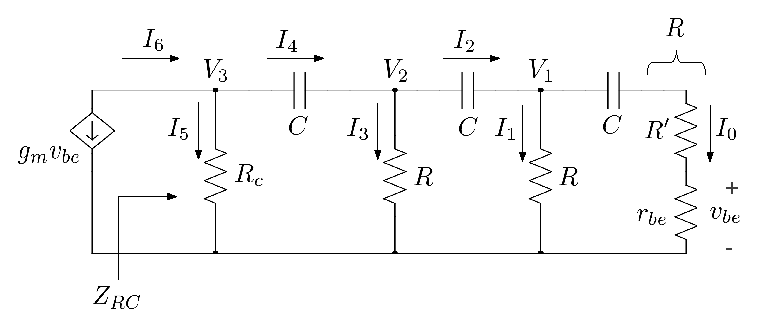
\includegraphics[scale=0.90]{phaseShiftOscillatorA}
\caption{مزاحمت-کپیسٹر مرتعش کی مساوات کا حصول}
\label{شکل_مزاحمت_کپیسٹر_مرتعش_الف}
\end{figure}
مرتعش ہر وقت اپنی قدرتی تعدد پر ارتعاش کرتا ہے۔یوں واپس کار کے کپیسٹر کی برقی رکاوٹ \عددیء{\frac{-j}{ \omega_0 C}} کو مساوات \حوالہ{مساوات_مزاحمت_کپیسٹر_مرتعش_قدرتی_تعداد_ارتعاش} کی مدد سے \عددیء{-j R \sqrt{6+4k}} لکھا جا سکتا ہے۔اس نتیجے کے مطابق اس برقی رکاوٹ کی قیمت \عددیء{C} کے بجائے مزاحمت \عددیء{R} پر منحصر ہے۔شکل \حوالہ{شکل_مزاحمت_کپیسٹر_مرتعش_الف} میں برقی رکاوٹ \عددیء{Z_{RC}} کی نشاندہی کی گئی ہے جو ٹرانزسٹر پر بطور برقی بوجھ لدا ہے۔یوں \عددیء{Z_{RC}} کی قیمت بھی \عددیء{C} پر منحصر نہیں ہو گی۔اگرچہ واپس کار کے کسی بھی مزاحمت یا کپیسٹر کو تبدیل کرتے ہوئے اس مرتعش کی قدرتی تعدد تبدیل کی جا سکتی ہے، حقیقت میں عموماً وسیح حدود کے درمیان تعدد تبدیل کرنے کی خاطر تینوں کپیسٹروں کو ایک ساتھ برابر تبدیل کیا جاتا ہے۔تینوں کپیسٹر یوں تبدیل کرنے سے \عددیء{Z_{RC}} ، جو کہ بنیادی ایمپلیفائر کا بوجھ ہے، تبدیل نہیں ہوتا اور یوں ارتعاشی لہر کا حیطہ بھی تبدیل نہیں ہوتا۔یہ مرتعش چند ہرٹز \عددیء{\si{\hertz}} سے کئی سو کلو ہرٹز  \عددیء{\si{\kilo \hertz}} تک کے ارتعاش پیدا کرنے کے لئے استعمال کیا جاتا ہے۔میگا ہرٹز \عددیء{\si{\mega \hertz}} کے حدود میں اسے دیگر اقسام کے امالہ-کپیسٹر \عددیء{LC} مرتعشوں پر فوقیت حاصل نہیں۔

آئیں اب \عددیء{Z_{RC}} کی اصل قیمت حاصل کریں۔شکل سے ظاہر ہے کہ
\begin{align*}
Z_{RC}=\frac{V_3}{I_6}
\end{align*}
کے برابر ہے۔مساوات \حوالہ{مساوات_مزاحمت_کپیسٹر_دباو_تین} اور مساوات \حوالہ{مساوات_مزاحمت_کپیسٹر_بار_کی_رو} کی مدد سے
\begin{align*}
Z_{RC}=\frac{I_0 \left(R+\frac{6}{j \omega C}+\frac{5}{\left(j \omega C \right )^2 R} +\frac{1}{\left(j \omega C \right )^3 R^2}\right)}{I_0 \left( \frac{1}{k}+3 -\frac{\left(\frac{5}{k}+1 \right )}{\left(\omega C R \right)^2}+j \left [\frac{1}{\left (\omega C R \right)^3 k}  -\frac{\left(\frac{6}{k}+4 \right)}{\omega C R}\right] \right )}
\end{align*}
مساوات \حوالہ{مساوات_مزاحمت_کپیسٹر_مرتعش_قدرتی_تعداد_ارتعاش} میں دئے \عددیء{\omega} کی قیمت اس مساوات میں استعمال کرتے ہوئے
\begin{align*}
Z_{RC}&=\frac{ R+\frac{6 CR\sqrt{6+4k}}{j C}+\frac{5 \left(CR\sqrt{6+4k} \right)^2}{\left(j C \right )^2 R} +\frac{\left(CR\sqrt{6+4k} \right)^3}{\left(j C \right )^3 R^2}}{  \frac{1}{k}+3 -\frac{\left(\frac{5}{k}+1 \right ) \left(CR\sqrt{6+4k} \right)^2}{\left( C R \right)^2}+j \left [\frac{\left(CR\sqrt{6+4k} \right)^3}{\left (C R \right)^3 k}  -\frac{\left(\frac{6}{k}+4 \right)\left(CR\sqrt{6+4k} \right)}{C R}\right] }\\
&=\frac{-R \left[ 1+\frac{6\sqrt{6+4k}}{j }+\frac{5 \left(\sqrt{6+4k} \right)^2}{\left(j \right )^2} +\frac{\left(\sqrt{6+4k} \right)^3}{\left(j \right )^3} \right]}{\frac{29}{k}+23 +4k}
\end{align*}
حاصل ہوتا ہے۔اگر  \عددیء{\beta} مساوات \حوالہ{مساوات_مرتعش_مزاحمت_کپیسٹر_درکار_افزائش} کے مطابق ہو تب
\begin{align}
Z_{RC}=\frac{R}{\beta} \left[ 29+20k -j 4 k \sqrt{6+4k}\right]
\end{align}
حاصل ہوتا ہے۔

\begin{figure}
\centering
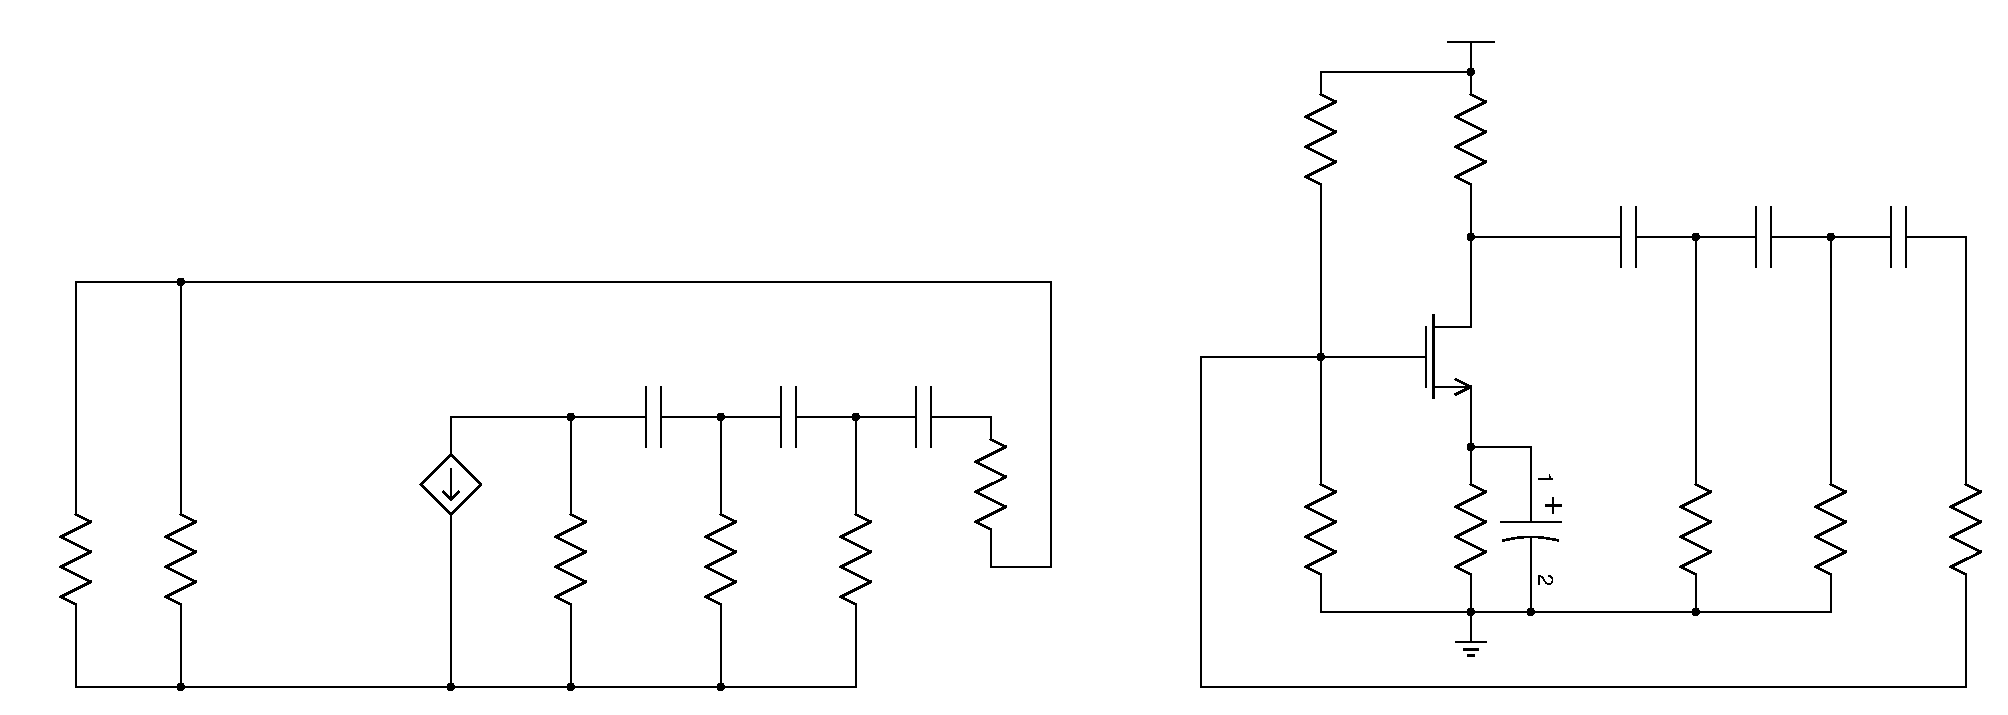
\includegraphics[scale=0.90]{phaseShiftMosfetOscillator}
\caption{مزاحمت-کپیسٹر ماسفیٹ مرتعش}
\label{شکل_مزاحمت_کپیسٹر_ماسفیٹ_مرتعش}
\end{figure}
%
شکل \حوالہ{شکل_مزاحمت_کپیسٹر_ماسفیٹ_مرتعش} الف میں ماسفیٹ سے \عددیء{RC} مرتعش کا حصول دکھایا گیا ہے۔شکل  ب میں اسی کا مساوی دور دکھایا گیا ہے۔جیسے آپ دیکھ سکتے ہیں یہ بالکل دو جوڑ ٹرانزسٹر کے دور کے طرح کا ہی ہے۔حقیقی دور میں \عددیء{R'} کے استعمال کی ضرورت نہیں ہوتی چونکہ \عددیء{R_1} اور \عددیء{R_2} کو یوں رکھنا ممکن ہو گا کہ یہ ماسفیٹ کو یک سمتی مائل کرنے کے ساتھ ساتھ \عددیء{R=R_m} کے شرط کو بھی پورا کرے جہاں \عددیء{R_m = \frac{R_1 R_2}{R_1+R_2}} کے برابر ہے۔
%================
\حصہ{وائن مرتعش}
شکل \حوالہ{شکل_مرتعش_وائن} میں \اصطلاح{وائن مرتعش}\فرہنگ{وائن مرتعش}\فرہنگ{مرتعش!وائن}\حاشیہب{Wien bridge oscillator}\فرہنگ{Wien bridge oscillator} دکھایا گیا ہے۔وائن مرتعش\حاشیہد{اس مرتعش کو میکس وائن نے دریافت کیا۔} پر پہلے بغیر حل کئے غور کرتے ہیں۔
\begin{figure}
\centering
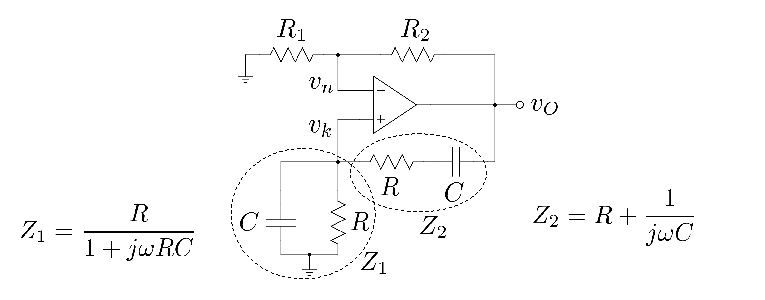
\includegraphics[scale=0.90]{wienBridgeOscillator}
\caption{وائن مرتعش}
\label{شکل_مرتعش_وائن}
\end{figure}

آپ جانتے ہیں کہ یک سمتی رو پر کپیسٹر کھلے سرے کردار ادا کرتا ہے۔یوں اگر \عددیء{v_O} برقرار کسی مثبت برقی رو پر رہے تب \عددیء{Z_2} کھلے سرے کردار ادا کرے گا جبکہ \عددیء{Z_1} بطور مزاحمت \عددیء{R} کردار ادا کرے گا۔یوں \عددیء{v_k} برقی زمین پر رہے گا اور \عددیء{v_k=0} ہو گا۔اس کے برعکس \عددیء{R_1} اور \عددیء{R_2} حسابی ایمپلیفائر کے مثبت خارجی برقی دباو \عددیء{v_O} سے \عددیء{v_n=\tfrac{R_1 v_O}{R_1+R_2}} پیدا کریں گے جو کہ مثبت برقی دباو ہو گا۔ایسی صورت میں \عددیء{v_n > v_k} ہے اور حسابی ایمپلیفائر کا خارجی اشارہ \عددیء{v_O} برقرار مثبت نہیں رہ سکتا اور یہ جلد از جلد منفی ہونے کی کوشش کرے گا ۔آئیں اب تصور کریں کہ \عددیء{v_O} برقرار کسی منفی برقی دباو پر رہتا ہے۔اس مرتبہ بھی \عددیء{v_k=0} ہی حاصل ہوتا ہے البتہ منفی \عددیء{v_O} کی صورت میں \عددیء{v_n=\tfrac{R_1 v_O}{R_1+R_2}} بھی منفی برقی دباو ہو گا اور یوں \عددیء{v_k > v_n} ہو گا۔ایسی صورت میں حسابی ایمپلیفائر  کا خارجی اشارہ برقرار منفی نہیں رہ سکتا اور یہ جلد از جلد مثبت ہونے کی کوشش کرے گا۔مندرجہ بالا تبصرے سے یہ حقیقت اجاگر ہوئی کہ \عددیء{v_O} برقرار نہ مثبت اور نا ہی منفی برقی دباو پر ٹھر سکتا ہے بلکہ یہ ارتعاش پذیر رہتا ہے۔

اگر \عددیء{v_O=0} تصور کیا جائے تب \عددیء{v_k=v_n=0} ہی حاصل ہوتے ہیں اور \عددیء{v_O} برقرار برقی زمین پر ہی رہے گا۔یہ صورت حال نا پائیدار ہے۔برقی ادوار میں مسلسل برقی شور پایا جاتا ہے جس کی وجہ سے کسی بھی مقام پر پائے جانے والے برقی دباو میں لمحہ با لمحہ باریک تبدیلیاں پیدا ہوتی ہیں۔یوں \عددیء{v_k} اور \عددیء{v_n} زیادہ دیر مکمل طور پر برابر برقی دباو پر نہیں رہ سکتے اور جلد ہی لمحاتی طور پر \عددیء{v_k>v_n} اور یا \عددیء{v_k<v_n} ہو جائے گا۔ایسا ہوتے ہی \عددیء{v_O} حرکت میں آئے گا اور دور ارتعاش پذیر ہو جائے گا۔آئیں اب وائن مرتعش کا تحلیلی تجزیہ کریں

وائن مرتعش کو دیکھتے ہوئے ہم لکھ سکتے ہیں۔
\begin{gather}
\begin{aligned}\label{مساوات_وائن_مرتعش_برقی_دباو}
v_n&=\left(\frac{R_1}{R_1+R_2}\right) v_O\\
v_k&=\left(\frac{Z_1}{Z_1+Z_2}\right) v_O
\end{aligned}
\end{gather} 
جہاں
\begin{gather}
\begin{aligned}\label{مساوات_وائن_مرتعش_مقاومت}
Z_1&=\frac{R}{1+j \omega R C}\\
Z_2&=R+\frac{1}{j \omega C}\\
&=\frac{1+j \omega R C}{j \omega C}
\end{aligned}
\end{gather}
کے برابر ہیں۔مساوات \حوالہ{مساوات_وائن_مرتعش_مقاومت} کو مساوات \حوالہ{مساوات_وائن_مرتعش_برقی_دباو} میں پُر کرتے ہوئے اور \عددیء{v_k=v_n} لکھتے ہوئے
\begin{align*}
\left(\frac{R_1}{R_1+R_2}\right) v_O=\left(\frac{\frac{R}{1+j \omega R C}}{\frac{R}{1+j \omega R C}+\frac{1+j \omega R C}{j \omega C}}\right) v_O
\end{align*}
حاصل ہوتا ہے۔اس کو حل کرتے ہوئے
\begin{align*}
\frac{R_1}{R_1+R_2}&=\frac{j \omega R C}{j \omega R C +\left(1+j \omega R C \right)^2}\\
&=\frac{j \omega R C}{j 3 \omega R C +1-\omega^2 R^2 C^2}
\end{align*}
یعنی
\begin{align}
R_1 \left[j 3 \omega R C +1-\omega^2 R^2 C^2 \right]=j \omega R C\left(R_1+R_2 \right)
\end{align}
ملتا ہے۔اس مساوات کے حقیقی اور خیالی اجزاء علیحدہ کرتے ہوئے
\begin{align*}
R_1\left(1-\omega^2 R^2 C^2 \right)=0\\
j 3 \omega R C R_1=j\omega R C \left(R_1+R_2 \right)
\end{align*}
حاصل ہوتا ہے جس سے
\begin{gather}
\begin{aligned}\label{مساوات_وائن_مرتعش_تخلیقی_مساوات}
\omega=\omega_o &=\frac{1}{R C}\\
R_2&=2R_1
\end{aligned}
\end{gather} 
حاصل ہوتا ہے۔مساوات \حوالہ{مساوات_وائن_مرتعش_تخلیقی_مساوات} وائن مرتعش کے شرائط بیان کرتے ہیں۔ان شرائط کے مطابق وائن مرتعش کی قدرتی تعدد \عددیء{\tfrac{1}{R C}} کے برابر ہے اور یہ اس وقت ارتعاش کرے گا جب \عددیء{R_2} کی قیمت \عددیء{R_1} کے دگنا ہو۔

وائن مرتعش کو مثبت حسابی ایمپلیفائر تصور کیا جا سکتا ہے جہاں \عددیء{v_k} اس کا داخلی اشارہ جبکہ \عددیء{\tfrac{R_1+R_2}{R_1}} اس کی افزائش \عددیء{A_v} ہے۔\عددیء{R_2=2 R_1} کی صورت میں \عددیء{A_v=\SI{3}{\volt \per \volt}} کے برابر ہو گا۔اس قیمت سے کم افزائش پر مرتعش ارتعاش پذیر نہ ہو پائے گا۔مستحکم مرتعش کے لئے ضروری ہے کہ افزائش اس قیمت سے قدر زیادہ ہو۔یوں حقیقت میں \عددیء{R_2 > 2 R_1} ہونا ضروری ہے۔اگر \عددیء{R_2} کی قیمت \عددیء{2 R_1} سے ذرہ سی زیادہ ہو تب مرتعش سائن نما لہر خارج کرتا ہے البتہ \عددیء{R_2 \gg 2 R_1} کی صورت میں \عددیء{A_v} کی قیمت بہت بڑھ جاتی ہے اور مرتعش مستطیل لہر خارج کرتا ہے۔

%=====================
\حصہ{\عددیء{nJFET} پر مبنی امالہ-کپیسٹر \عددیء{LC} ہمسُر مرتعش} \شناخت{حصہ_فیٹ_ہمسر_مرتعش}
مزاحمت-کپیسٹر مرتعش میں \عددیء{RC} کی کڑیاں جوڑ کر لہر کے زاویے میں \عددیء{\SI{180}{\degree}} کی تبدیلی پیدا کی گئی۔اس حصے میں مشترکہ امالہ (یعنی ٹرانسفارمر) کے استعمال سے \عددیء{\SI{180}{\degree}} کی تبدیلی حاصل کی جائے گی۔شکل \حوالہ{شکل_امالہ_کپیسٹر_مرتعش} میں \عددیء{L} اور \عددیء{L_g} کو قریب قریب رکھ کر مشترکہ امالہ \عددیء{M} حاصل کیا گیا ہے۔اس مرتعش کی کارکردگی سمجھنے کی خاطر تصور کریں کہ ماسفیٹ میں \عددیء{\omega_o} تعدد کی برقی رو پائی جاتی ہے جس کی وجہ سے اس پر نسب \عددیء{LC} پر اسی تعدد کی برقی دباو پیدا ہو گی۔مشترکہ امالہ کی وجہ سے  اس برقی دباو کا کچھ حصہ \عددیء{L_g} پر نمودار ہوتے ہوئے ماسفیٹ کو چلائے گا۔یوں گیٹ پر برقی دباو سے \عددیء{LC} پر برقی دباو پیدا ہوتا ہے اور \عددیء{LC} پر برقی دباو کی وجہ سے گیٹ پر برقی دباو پیدا ہوتا ہے۔یہ نا ختم ہونے والا سلسلہ یوں برقرار رہے گا۔آئیں اب اس مرتعش پر تحلیلی بحث کریں۔

\عددیء{nJFET} کا گیٹ کھلے سرے  کردار ادا کرتا ہے لہٰذا \عددیء{L_g} میں صفر برقی رو گزرے گا۔اس صورت میں اگر \عددیء{L} پر برقی دباو \عددیء{v_L} پایا جائے تو \عددیء{L_g} پر مشترکہ امالہ \عددیء{M} کی وجہ سے \عددیء{v_M} پیدا ہو گا جہاں
\begin{figure}
\centering
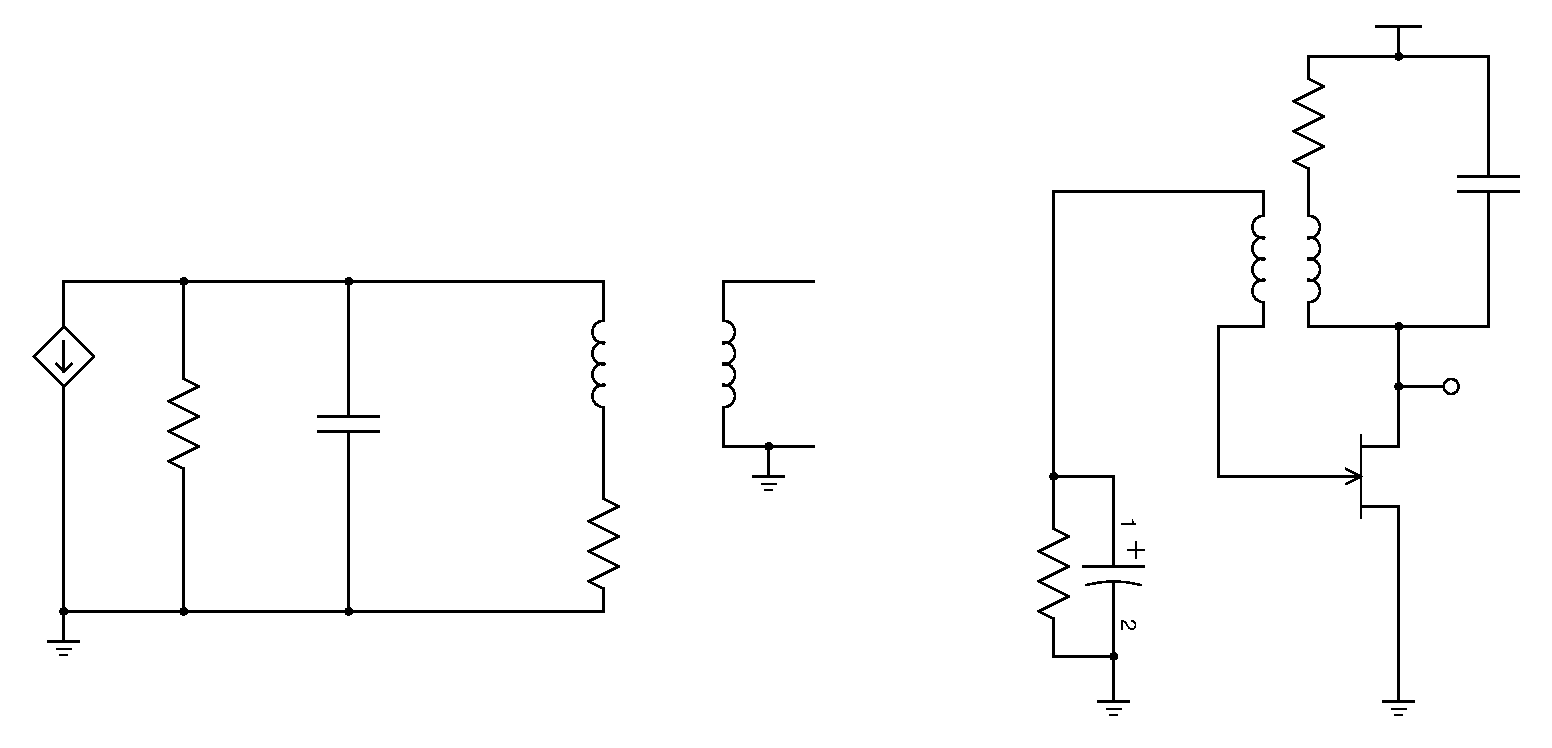
\includegraphics[scale=0.90]{tunedOscillator}
\caption{امالہ-کپیسٹر مرتعش}
\label{شکل_امالہ_کپیسٹر_مرتعش}
\end{figure}
%
\begin{align}
\frac{v_M}{v_L}=\frac{M}{L}
\end{align}
کے برابر ہو گا۔مشترکہ امالہ میں برقی طاقت کے  ضیاع کو مزاحمت \عددیء{r} سے ظاہر کیا گیا ہے۔مشترکہ امالہ میں نقطوں سے ہم زاویہ سرے دکھائے جاتے ہیں۔یوں اگر \عددیء{L} پر برقی دباو کا مثبت سرا نقطے  کی جانب ہو تو \عددیء{L_g} پر بھی برقی دباو کا مثبت سرا نقطے  کی جانب ہو گا۔شکل سے واضح ہے کہ \عددیء{v_{gs}=-v_M} کے برابر ہے۔ یوں
\begin{align} \label{مساوات_مشترکہ_برقی_دباو}
v_{gs}=-\left(\frac{M}{L} \right) v_L
\end{align} 
ہو گا۔

شکل  ب میں \عددیء{v_o=-g_m v_{gs} Z} کے برابر ہے جسے \عددیء{g_m v_{gs}=-\frac{v_o}{Z}} لکھا جا سکتا ہے جہاں
\begin{align*}
\frac{1}{Z}=\frac{1}{r_o}+j \omega C +\frac{1}{r +j \omega L}
\end{align*}
کے برابر ہے۔یوں
\begin{align} \label{مساوات_امالہ_کپیسٹر_مرتعش_برقی_رو}
g_m v_{gs}=-\left(\frac{1}{r_o}+j \omega C +\frac{1}{r +j \omega L} \right) v_o
\end{align}
 ہو گا۔\عددیء{r} اور \عددیء{L} سلسلہ وار جڑے ہیں اور یوں
\begin{align}
v_L =\left( \frac{j \omega L}{r+j \omega L} \right) v_o
\end{align}
کے برابر ہے۔یوں مساوات \حوالہ{مساوات_مشترکہ_برقی_دباو} کو
\begin{align}
v_{gs}=-\left(\frac{M}{L} \right) \left( \frac{j \omega L}{r+j \omega L} \right) v_o
\end{align}
اور مساوات \حوالہ{مساوات_امالہ_کپیسٹر_مرتعش_برقی_رو} کو یوں لکھ سکتے ہیں۔
\begin{align*}
-g_m \left(\frac{M}{L} \right) \left( \frac{j \omega L}{r+j \omega L} \right) v_o=-\left(\frac{1}{r_o}+j \omega C +\frac{1}{r +j \omega L} \right) v_o
\end{align*}
دونوں جانب \عددیء{-v_o} کو کاٹتے ہوئے \عددیء{(r+j \omega L)} سے ضرب دیتے ہیں۔
\begin{gather}
\begin{aligned} \label{مساوات_امالہ_کپیسٹر_مرتعش_مساوات}
j \omega M g_m &=\frac{r+j \omega L}{r_o}+j \omega C \left(r+j \omega L \right) +1  \\
&=\frac{r}{r_o}+\frac{j \omega L }{r_o}+j \omega C r-\omega^2 LC+1 
\end{aligned}
\end{gather}
اس مساوات میں حقیقی اور خیالی جزو علیحدہ کئے جا سکتے ہیں۔حقیقی جزو حل کرتے قدرتی تعدد \عددیء{\omega_0} کی قیمت حاصل ہوتی ہے
\begin{gather}
\begin{aligned}
\frac{r}{r_o}-\omega_0^2 LC +1 =0 \\
\omega_0 = \sqrt{\frac{1}{LC} \left(\frac{r}{r_o}+1 \right)}
\end{aligned}
\end{gather}
حقیقت میں مشترکہ امالہ کی مزاحمت \عددیء{r} کی قیمت ماسفیٹ کے مزاحمت \عددیء{r_o} سے نہایت کم ہوتی ہے یعنی \عددیء{r \ll r_o} ہوتا ہے۔ یوں مندرجہ بالا مساوات کے مطابق قدرتی تعدد کی قیمت تقریباً \عددیء{LC} کی قدرتی تعدد کے برابر ہوتی ہے یعنی
\begin{align}
\omega_0 = \frac{1}{\sqrt{LC}}
\end{align}
جہاں تقریباً کی جگہ برابر کا نشان استعمال کیا گیا ہے۔اس اتفاقی اور دلچسپ نتیجے کے مطابق یہ مرتعش متوازی جڑے \عددیء{LC} کی قدرتی تعدد پر ارتعاش کرتا ہے۔اسی نتیجے کی بنا پر اس مرتعش کو \عددیء{LC} \اصطلاح{ہمسُر مرتعش}\فرہنگ{ہمسر مرتعش}\فرہنگ{مرتعش!ہمسر}\فرہنگ{tuned oscillator}\حاشیہب{tuned oscillator} کہا جاتا ہے۔اس مرتعش کی تعدد کپیسٹر \عددیء{C} کی قیمت تبدیل کرتے ہوئے تبدیل کی جا سکتی ہے۔

مساوات \حوالہ{مساوات_امالہ_کپیسٹر_مرتعش_مساوات} میں خیالی جزو حل کرتے ہوئے کم سے کم \عددیء{g_m} کی قیمت حاصل ہوتی ہے یعنی
\begin{gather}
\begin{aligned}\label{مساوات_مرتعش_ہمسر_حقیقی_اجزاء}
\omega M g_m &= \frac{\omega L}{r_o}+\omega C r\\
g_m&=\frac{1}{M} \left(\frac{L}{r_o}+Cr \right )
\end{aligned}
\end{gather}
\عددیء{r} کو نظر انداز کرتے ہوئے ہم دیکھتے ہیں کہ مرتعش \عددیء{\omega_0} پر ارتعاش کرے گا۔\عددیء{\omega_0} پر متوازی جڑے \عددیء{LC} کی برقی رکاوٹ لامحدود ہو گی اور بنیادی ایمپلیفائر کے لئے ہم
\begin{align*}
v_o=-g_m v_{gs} r_o
\end{align*}
لکھ سکتے ہیں۔یوں 
\begin{align*}
A_v=\frac{v_o}{v_{gs}}=-g_m r_o
\end{align*}
ہو گا۔لامحدود بوجھ پر افزائش کی حتمی قیمت کو \عددیء{\mu} لکھتے ہوئے یعنی \عددیء{\mu=g_m r_o} لیتے ہوئے مساوات \حوالہ{مساوات_مرتعش_ہمسر_حقیقی_اجزاء} میں \عددیء{r_o} کی جگہ \عددیء{\frac{\mu}{g_m}} لکھتے ہوئے حل کرتے ہیں۔
\begin{align*}
g_m M&= \frac{L}{r_o}+Cr \\
g_m M&=\frac{L g_m}{\mu}+Cr\\
g_m&=\frac{\mu C r}{\mu M-L}
\end{align*}
حقیقی مرتعش کی \عددیء{g_m} اس سے زیادہ ہو گی۔
%
\جزوحصہ{خود-مائل دور}
شکل \حوالہ{شکل_امالہ_کپیسٹر_مرتعش} میں \عددیء{nJFET} کے مائل ہونے پر غور کرتے ہیں۔تصور کریں کہ  مرتعش ارتعاش پذیر ہے۔ یوں مشترکہ امالہ کی وجہ سے  گیٹ پر سائن نما برقی دباو \عددیء{V_p \sin \omega t} پایا جائے گا۔\عددیء{nJFET} کے گیٹ پر جب بھی مثبت برقی دباو لاگو کی جائے یہ کسی بھی ڈایوڈ کی طرح سیدھا مائل ہو جاتا ہے۔گیٹ کا ڈایوڈ، کپیسٹر \عددیء{C_g} اور مزاحمت \عددیء{R_g} بطور چوٹی حاصل کار کردار ادا کرتے ہیں جس پر حصہ \حوالہ{حصہ_چوٹی_حاصل_کار} میں تفصیلاً غور کیا گیا ہے۔یوں کپیسٹر \عددیء{C_g} پر برقی دباو، گیٹ پر پائے جانے والے سائن نما لہر کے چوٹی برابر ہو جائے گا یعنی اس پر \عددیء{V_p} برقی دباو پایا جائے گا۔جیسا شکل میں دکھایا گیا ہے، کپیسٹر پر برقی دباو کا مثبت سرا برقی زمین کے ساتھ جڑا ہے۔یوں گیٹ پر \عددیء{-V_p} برقی دباو پایا جائے گا جو \عددیء{nJFET} کو مائل کرتا ہے۔\عددیء{R_g} کی قیمت یوں رکھی جاتی ہے کہ  لہر کے ایک دوری عرصے میں \عددیء{C_g} پر برقی دباو برقرار رہے۔ایسا کرنے کی خاطر \عددیء{R_g C_g \gg \frac{1}{f}}  رکھا جاتا ہے جہاں \عددیء{f} لہر کی تعدد ہے۔اس مرتعش کی تعدد حاصل کرتے وقت تصور کیا گیا تھا کہ گیٹ پر برقی رو کا گزر ممکن نہیں۔یہاں ہم دیکھتے ہیں کہ \عددیء{nJFET} کو مائل کرنے کی خاطر گیٹ کے ڈایوڈ کا سیدھا مائل ہونا لازم ہے۔چونکہ لہر کی چوٹی پر نہایت کم دورانیہ کے لئے گیٹ سیدھا مائل ہوتا ہے جبکہ بقایا تمام وقت یہ الٹ مائل رہتا ہے لہٰذا گیٹ کو کھلے سرے تصور کیا جا سکتا ہے۔

جس لمحہ مرتعش کو برقی طاقت \عددیء{V_{DD}} مہیا کیا جائے اس لمحہ \عددیء{C_g} پر صفر برقی دباو پایا جاتا ہے۔یوں  \عددیء{nJFET} زیادہ \عددیء{i_{DS}} گزرنے دیتا ہے جس سے اس کی \عددیء{g_m} کی قیمت بھی زیادہ ہوتی ہے۔زیادہ \عددیء{g_m} کی وجہ سے دور کا ارتعاش پذیر ہونا ممکن ہوتا ہے۔تصور  کریں کہ ایسا ہی ہوتا ہے۔\عددیء{g_m} کی زیادہ قیمت کی وجہ سے ارتعاشی لہر کا حیطہ بڑھتا جاتا ہے جس سے \عددیء{C_g} پر برقی دباو \عددیء{V_p} بھی بڑھتا جاتا ہے جو کہ گیٹ کو زیادہ سے زیادہ منفی کرتے ہوئے \عددیء{i_{DS}} کی قیمت کو کم کرتا ہے۔کم \عددیء{i_{DS}} کی وجہ سے \عددیء{g_m} کی قیمت بھی کم ہوتی ہے۔آخر کار دور ایسی توازن اختیار  کر لیتا ہے جہاں ارتعاشی لہر کا حیطہ برقرار رہتا ہے۔ 

\حصہ{ٹرانزسٹر ہمسُر مرتعش}
حصہ \حوالہ{حصہ_فیٹ_ہمسر_مرتعش} میں \عددیء{nJFET} کا کم تعددی ریاضی نمونہ استعمال کرتے  ہوئے مرتعش کو حل کرنا دکھایا گیا جس میں ٹرانسفارمر کو بطورِ مشترکہ امالہ تصور کیا گیا۔اس حصے میں دو جوڑ ٹرانزسٹر کا بلند تعددی ریاضی نمونہ اور ٹرانسفارمر کے مساوات استعمال کرتے ہوئے \اصطلاح{ہمسر مرتعش}\فرہنگ{ہمسر مرتعش}\حاشیہب{tuned oscillator}\فرہنگ{tuned oscillator} کا حل دکھایا جائے گا۔ظاہر ہے  کہ فیٹ پر مبنی مرتعش کو بھی اسی طرح حل کیا جا سکتا ہے۔بلند تعدد پر ٹرانزسٹر (یا فیٹ) کے بلند تعدد ریاضی نمونہ ہی سے درست جوابات حاصل ہوتے ہیں لہٰذا بلند تعدد پر چلنے والے مرتعش کو حل کرتے ہوئے ٹرانزسٹر (یا فیٹ) کا بلند تعدد ریاضی نمونہ استعمال کرنا ضروری ہے۔
\begin{figure}
\centering
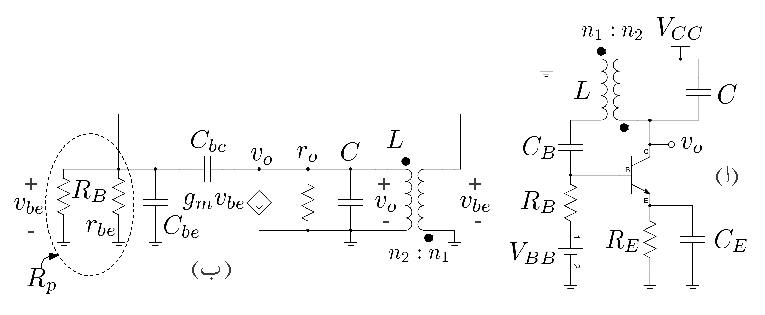
\includegraphics[scale=0.90]{transistorTunedOscillator}
\caption{ٹرانزسٹر ہمسُر مرتعش}
\label{شکل_ٹرانزسٹر_ہمسر_مرتعش}
\end{figure}
%
\begin{figure}
\centering
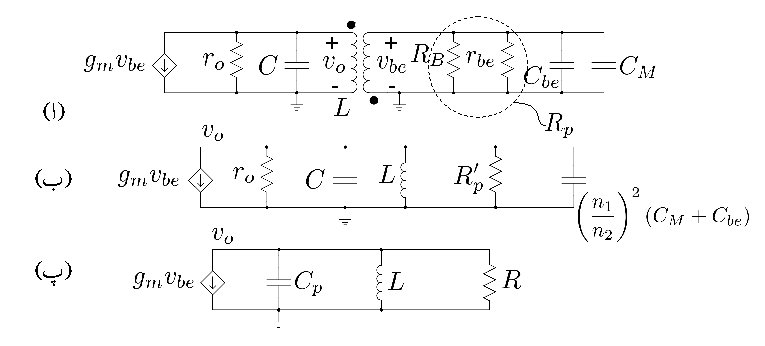
\includegraphics[scale=0.90]{transistorTunedOscillatorEquivalent}
\caption{ٹرانزسٹر ہمسُر مرتعش کا باریک اشاراتی مساوی دور}
\label{شکل_ٹرانزسٹر_ہمسر_مرتعش_مساوی}
\end{figure}
%
شکل \حوالہ{شکل_ٹرانزسٹر_ہمسر_مرتعش} الف میں \اصطلاح{ٹرانزسٹر ہمسُر مرتعش} دکھایا گیا ہے۔ٹرانزسٹر کا بلند تعددی ریاضی نمونہ استعمال کرتے ہوئے شکل  ب میں اسی کا مساوی دور دکھایا گیا ہے جس میں \عددیء{C_B} اور \عددیء{C_E} کو لامحدود تصور کیا گیا ہے۔\اصطلاح{مسئلہ ملر}\فرہنگ{مسئلہ ملر}\فرہنگ{Miller theorem}\حاشیہب{Miller theorem} کی مدد سے \عددیء{C_{bc}} کا مساوی ملر کپیسٹر \عددیء{C_M}استعمال کرتے ہیں۔یوں \عددیء{C_{be}} اور \عددیء{C_M} متوازی جڑ جاتے ہیں۔شکل \حوالہ{شکل_ٹرانزسٹر_ہمسر_مرتعش_مساوی} الف میں ایسا دکھایا گیا ہے جہاں شکل کو قدر بہتر طرز پر بنایا گیا ہے۔ٹرانسفارمر کے \عددیء{n_1} جانب برقی رکاوٹ کا \عددیء{n_2} جانب عکس لیتے ہیں۔ایسا کرتے وقت برقی رکاوٹ کو \عددیء{\left(\frac{n_2}{n_1} \right)^2} سے ضرب دیا جاتا ہے۔یوں متوازی جڑے مزاحمت \عددیء{r_{be}} اور \عددیء{R_B} کو \عددیء{R_p} لکھتے ہوئے ٹرانسفارمر کی دوسری جانب منتقل کرتے \عددیء{R_p'} حاصل ہوتا ہے جہاں
\begin{align*}
R_p'=\left(\frac{n_2}{n_1} \right)^2 R_p
\end{align*}
کے برابر ہے۔\عددیء{C_{be}} اور \عددیء{C_M} متوازی جڑے ہیں لہٰذا ان کا مجموعہ \عددیء{C_{be}+C_M} اور برقی رکاوٹ \عددیء{\tfrac{1}{j \omega (C_{be}+C_M)}} کے برابر ہے۔اس کا عکس
\begin{align*}
\left(\frac{n_2}{n_1} \right)^2  \times \frac{1}{j \omega \left(C_{be}+C_M \right)}
\end{align*}
ہو گا جس کو
\begin{align*}
\frac{1}{j \omega \left[\frac{n_1^2}{n_2^2} \left(C_{be}+C_M \right)\right]}
\end{align*}
لکھا جا سکتا ہے۔یوں \عددیء{C_{be}+C_M} کا عکس
 \begin{align*}
\left(\frac{n_1}{n_2} \right)^2 \left(C_{be}+C_M \right)
\end{align*}
حاصل ہوتا ہے ہے جو \عددیء{C} کے متوازی پایا جاتا ہے۔ان تمام متوازی جڑے کپیسٹروں کو \عددیء{C_p} لکھا گیا ہے جہاں
\begin{align*}
C_p = C +\left(\frac{n_1}{n_2} \right)^2 \left(C_{be}+C_M \right)
\end{align*}
کے برابر ہے۔اسی طرح متوازی جڑے \عددیء{r_o} اور \عددیء{R_p'} کے مجموعے کو \عددیء{R} لکھا جا سکتا ہے۔ایسا کرتے ہوئے شکل  ب سے شکل  پ حاصل ہوتا ہے۔


شکل  پ کو حل کرتے ہیں جس میں
\begin{align*}
\frac{1}{Z}=j \omega C_p +\frac{1}{j \omega L} +\frac{1}{R}
\end{align*}
کے برابر ہے۔یوں \عددیء{v_o = -g_m v_{be} Z} کے برابر ہو گا جسے \عددیء{-g_m v_{be} = \frac{v_o}{Z}} لکھا جا سکتا ہے یعنی
\begin{align} \label{مساوات_ہمسر_الف}
-g_m v_{be}=\left(j \omega C_p +\frac{1}{j \omega L} +\frac{1}{R} \right) v_o
\end{align}
ٹرانسفارمر کے دو جانب برقی دباو کی شرح ان دو جانب لچھوں کے چکر کی شرح کے برابر ہوتا ہے۔مزید اگر ایک جانب برقی دباو کا مثبت سرا ٹرانسفارمر کی علامت پر دکھائے نقطے  کی طرف ہو تو دوسری جانب بھی برقی دباو کا مثبت سرا اس جانب نقطے  کی طرف کو ہو گا۔ان دو حقائق سے
\begin{align*}
v_{be}=-\left(\frac{n_1}{n_2} \right) v_o
\end{align*}
حاصل ہوتا ہے جہاں منفی کی علامت اس بات کو دکھلاتا ہے کہ ہم نے ٹرانسفارمر کے ایک جانب \عددیء{v_o} کا مثبت سرا نقطے  کی جانب جبکہ دوسری جانب \عددیء{v_{be}} کا مثبت سرا بغیر نقطے  کی طرف رکھا ہے۔ایسا کرنے سے اشارے میں \عددیء{\SI{180}{\degree}} کی تبدیلی پیدا کی جاتی ہے جو کہ \عددیء{RC} مرتعش میں تین کڑی \عددیء{RC} سے حاصل کی گئی تھی۔

یوں مساوات \حوالہ{مساوات_ہمسر_الف} سے حاصل ہوتا ہے 
\begin{align*}
g_m \left(\frac{n_1}{n_2} \right) v_o &=\left(j \omega C_p +\frac{1}{j \omega L} +\frac{1}{R} \right) v_o\\
g_m \left(\frac{n_1}{n_2} \right) &=\left(j \omega C_p +\frac{1}{j \omega L} +\frac{1}{R} \right)
\end{align*}
اس مساوات کے خیالی اور حقیقی جزو علیحدہ کرتے ہیں۔خیالی جزو سے حاصل ہوتا ہے
\begin{align}
\omega_o=\frac{1}{\sqrt{L C_p}}=\frac{1}{\sqrt{L \left[C+\left(\frac{n_1}{n_2}\right)^2 \left(C_{be}+C_M \right) \right]}}
\end{align}
جبکہ حقیقی جزو سے
\begin{align*}
g_m \left ( \frac{n_1}{n_2}\right)&=\frac{1}{R}=\left(\frac{n_1}{n_2} \right)^2  \times \frac{1}{R_p} +\frac{1}{r_o}
\end{align*}
لکھا جا سکتا ہے۔\عددیء{r_o} کی قیمت نسبتاً بہت زیادہ ہوتی ہے لہٰذا \عددیء{\tfrac{1}{r_o}} کو نظر انداز کرتے ہوئے
\begin{align*}
g_m R_p&=\frac{n_1}{n_2}
\end{align*}
حاصل ہوتا ہے۔چونکہ \عددیء{R_B} کی قیمت \عددیء{r_{be}} کے قیمت سے کئی درجے زیادہ ہوتی ہے لہٰذا
\begin{align*}
R_p=\frac{R_B r_{be}}{R_B+r_{be}} \approx r_{be}
\end{align*}
ہوتا ہے  اور یوں
\begin{align*}
g_m r_{be}&=\frac{n_1}{n_2}
\end{align*}
لکھا جا سکتا ہے۔اس مساوات میں \عددیء{g_m r_{be}=\beta} کے استعمال سے
\begin{align}
\beta = \frac{n_1}{n_2}
\end{align}
حاصل ہوتا ہے۔

قدرتی تعدد \عددیء{\omega_o} پر متوازی جڑے \عددیء{L} اور \عددیء{C_p} کی برقی رکاوٹ لامحدود ہوتی ہے لہٰذا شکل \حوالہ{شکل_ٹرانزسٹر_ہمسر_مرتعش_مساوی} پ میں
\begin{align}
A_v=\frac{v_o}{v_{be}}=- g_m R 
\end{align}
کے برابر ہو گا۔یوں ملر کپیسٹر
\begin{align*}
C_M=C_{bc} \left(1+g_m R \right)
\end{align*}
کے برابر ہو گا۔

چونکہ \عددیء{\beta \gg 1} ہوتا ہے لہٰذا \عددیء{\tfrac{n_1}{n_2} \gg 1} ہو گا۔اگر \عددیء{\beta} کی قیمت \عددیء{\tfrac{n_1}{n_2}} سے معمولی زیادہ ہو تب مرتعش سائن نما لہر خارج کرتا ہے۔\عددیء{\beta \gg \tfrac{n_1}{n_2}} کی صورت میں ٹرانزسٹر غیر خطی خطے میں داخلی ہو گا اور یہ مستطیل برقی رو پیدا کرے گا البتہ \عددیء{L} اور \عددیء{C_p} اپنی قدرتی تعدد \عددیء{\omega_o} پر ارتعاش کرتے ہیں لہٰذا مرتعش سائن نما برقی دباو \عددیء{v_o} ہی خارج کرے گا۔
%========================

\حصہ{عمومی مرتعش}
شکل \حوالہ{شکل_عمومی_مرتعش} الف میں عمومی مرتعش دکھایا گیا ہے۔کئی قسم کے مرتعش اس عمومی طرز پر بنائے جاتے ہیں جہاں بنیادی ایمپلیفائر کسی بھی قسم کا ہو سکتا ہے مسئلاً حسابی ایمپلیفائر، دو جوڑ ٹرانزسٹر یا فیٹ پر مبنی ایمپلیفائر وغیرہ۔اس حصے میں بنیادی ایمپلیفائر کے داخلی مزاحمت کو لامحدود تصور کیا گیا ہے۔ایسا فیٹ پر مبنی ایمپلیفائر یا حسابی ایمپلیفائر کے استعمال سے ممکن ہے۔شکل  ب میں ایمپلیفائر کا تھونن مساوی دور استعمال کیا گیا ہے جہاں ایمپلیفائر کے خارجی مزاحمت کو \عددیء{R_o} لکھا گیا ہے۔ 
\begin{figure}
\centering
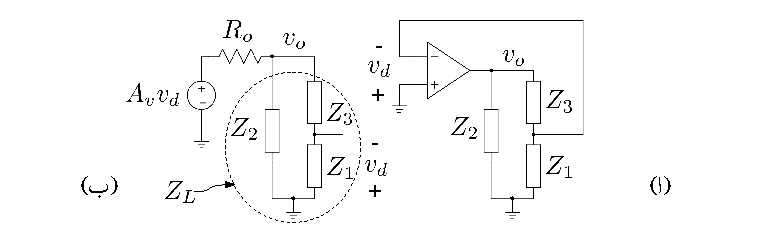
\includegraphics[scale=0.90]{generalOscillator}
\caption{عمومی مرتعش}
\label{شکل_عمومی_مرتعش}
\end{figure}
شکل  ب میں 
\begin{align*}
\frac{1}{Z_L}&=\frac{1}{Z_2}+\frac{1}{Z_1+Z_3}\\
Z_L&=\frac{Z_2 \left(Z_1+Z_3 \right)}{Z_1+Z_2+Z_3}
\end{align*}
کے برابر ہے۔یوں
\begin{align} \label{مساوات_عمومی_بار_دباو}
v_o = A_v v_d \left(\frac{Z_L}{R_o+Z_L} \right)
\end{align}
کے برابر ہو گا۔مزید یہ کہ \عددیء{Z_1} اور \عددیء{Z_3} کو سلسلہ وار جڑے تصور کرتے ہوئے
\begin{align}
v_d=-\left(\frac{Z_1}{Z_1+Z_3}\right) v_0
\end{align}
حاصل ہوتا ہے۔اس طرح مساوات \حوالہ{مساوات_عمومی_بار_دباو} سے
\begin{gather}
\begin{aligned} \label{مساوات_عمومی_رکاوٹ_مساوات}
v_o &= A_v \left(\frac{-Z_1}{Z_1+Z_3} \right) v_o \left(\frac{\frac{Z_2 \left(Z_1+Z_3 \right)}{Z_1+Z_2+Z_3}}{R_o+\frac{Z_2 \left(Z_1+Z_3 \right)}{Z_1+Z_2+Z_3}} \right)\\
1&=\frac{-A_v Z_1 Z_2 }{R_o \left(Z_1+Z_2+Z_3 \right)+Z_2 \left(Z_1+Z_3 \right )}
\end{aligned}
\end{gather}
حاصل ہوتا ہے۔

اس مرتعش میں \عددیء{Z} برقی رکاوٹ کو ظاہر کرتا ہے یوں امالہ کی صورت میں \عددیء{Z=j \omega L} ہو گا جبکہ کپیسٹر کی صورت میں  \عددیء{Z=-\frac{j}{\omega C}} ہو گا۔ہم \عددیء{\omega L} کو \عددیء{X_L} جبکہ \عددیء{-\frac{1}{\omega C}} کو \عددیء{X_C} لکھتے ہوئے \عددیء{Z=jX} لکھ سکتے ہیں جہاں مثبت \عددیء{X} امالہ کو ظاہر کرے گا جبکہ منفی \عددیء{X} کپیسٹر کو ظاہر کرے گا۔اس طرح  مساوات \حوالہ{مساوات_عمومی_رکاوٹ_مساوات} کو یوں لکھا جا سکتا ہے۔
\begin{gather}
\begin{aligned} \label{مساوات_عمومی_مرتعش_بنیادی}
1 &=\frac{-A_v j X_1 j X_2}{R_o \left(jX_1+jX_2+jX_3 \right)+jX_2 \left(jX_1+jX_3 \right )}\\
1&=\frac{A_v X_1 X_2 }{j R_o  \left(X_1+X_2+X_3 \right)-X_2 \left(X_1+X_3 \right )}
\end{aligned}
\end{gather}
اس مساوات کے بائیں ہاتھ صرف حقیقی مقداریں  جبکہ اس کے دائیں ہاتھ حقیقی اور خیالی دونوں مقداریں پائے جاتے ہیں۔مساوات کے دو اطراف صرف اور صرف اس صورت برابر ہو سکتے ہیں جب دونوں جانب مقداریں برابر ہوں۔چونکہ بائیں ہاتھ خیالی مقداریں نہیں پائے جاتے لہٰذا دائیں جانب خیالی مقداروں کی قیمت صفر ہو گی یعنی
\begin{align} \label{مساوات_عمومی_مرتعش_خیالی_جزو_صفر}
X_1+X_2+X_3=0
\end{align}
اور یوں مساوات \حوالہ{مساوات_عمومی_مرتعش_بنیادی} مندرجہ ذیل صورت اختیار کر لے گا۔
\begin{align*}
1&=\frac{-A_v X_1 X_2}{X_2 \left(X_1+X_3 \right )}=\frac{-A_v X_1}{X_1+X_3}
\end{align*}
مساوات \حوالہ{مساوات_عمومی_مرتعش_خیالی_جزو_صفر} سے \عددیء{X_1+X_3=-X_2} حاصل ہوتا ہے جسے مندرجہ بالا مساوات میں استعمال کرتے ہوئے
 \begin{align*}
1&=\frac{A_v X_1}{X_2}
\end{align*}
یعنی
\begin{align}\label{مساوات_مرتعش_عمومی_افزائش}
A_v &=\frac{X_2}{X_1}
\end{align}
دیتا ہے۔مساوات \حوالہ{مساوات_مرتعش_عمومی_افزائش} مرتعش کی درکار \عددیء{A_v} دیتا ہے۔ حقیقت میں \عددیء{A_v} اس قیمت سے زیادہ رکھا جائے گا۔اس مساوات میں \عددیء{A_v} مثبت قیمت رکھتا ہے لہٰذا مساواتی نشان کے دونوں جانب مثبت قیمتیں تب ممکن ہیں جب \عددیء{X_1} اور \عددیء{X_2} کی قیمتیں بھی یا تو دونوں مثبت ہوں اور یا پھر دونوں منفی ہوں۔یعنی یا یہ دونوں امالہ ہوں یا پھر دونوں کپیسٹر۔چونکہ مساوات \حوالہ{مساوات_عمومی_مرتعش_خیالی_جزو_صفر} کے تحت \عددیء{X_1+X_2=-X_3} ہو گا لہٰذا اگر \عددیء{X_1} اور \عددیء{X_2} دونوں امالہ ہوں تب \عددیء{X_3} کپیسٹر ہو گا اور ایسی صورت میں مرتعش کو \اصطلاح{ہارٹلے مرتعش}\فرہنگ{ہارٹلے مرتعش}\فرہنگ{مرتعش!ہارٹلے}\فرہنگ{Hartley oscillator}\حاشیہب{Hartley oscillator} پکارتے ہیں اور اگر \عددیء{X_1} اور \عددیء{X_2} دونوں کپیسٹر ہوں تب \عددیء{X_3} امالہ ہو گا اور ایسی صورت میں اسے \اصطلاح{کالپٹس مرتعش}\فرہنگ{کالپٹس مرتعش}\فرہنگ{مرتعش!کالپٹس}\فرہنگ{Colpitts oscillator}\حاشیہب{Colpitts oscillator} پکارا جاتا ہے۔\حاشیہد{رالف ہارٹلے نے ہارٹلے مرتعش جبکہ ایڈون ہنری کالپٹس نے کالپٹس مرتعش کا دور دریافت کیا۔}

اگر \عددیء{X_1} اور \عددیء{X_2} دونوں امالہ ہوں تب مساوات \حوالہ{مساوات_عمومی_مرتعش_خیالی_جزو_صفر} کو
\begin{align*}
j \omega L_1 +j \omega L_2 -\frac{j}{\omega C_3}=0
\end{align*}
لکھا جا سکتا ہے جس سے
\begin{align}\label{مساوات_مرتعش_ہارٹلے_قدرتی_تعدد}
\omega_0=\frac{1}{\sqrt{\left(L_1+L_2 \right) C}}
\end{align}
حاصل ہوتا ہے۔اسی طرح اگر \عددیء{X_1} اور \عددیء{X_2} کپیسٹر ہوں تب مساوات \حوالہ{مساوات_عمومی_مرتعش_خیالی_جزو_صفر} کو
\begin{align*}
-\frac{j}{\omega C_1}-\frac{1}{\omega C_2}+j \omega L_3=0
\end{align*}
لکھا جا سکتا ہے جس سے
\begin{align}\label{مساوات_مرتعش_کالپٹس_قدرتی_تعدد}
\omega_0=\frac{1}{\sqrt{L C}}
\end{align}
حاصل ہوتا ہے جہاں
\begin{align}
C=\frac{C_1 C_2}{C_1 + C_2}
\end{align}
یعنی \عددیء{C_1} اور \عددیء{C_2} کی سلسلہ وار جڑی کل کپیسٹر ہے۔

\حصہ{ہارٹلے اور کالپٹس مرتعش}
شکل \حوالہ{شکل_مرتعش_ہارٹلے_کالپٹس} میں ٹرانزسٹر ایمپلیفائر استعمال کرتے ہوئے ہارٹلے اور کالپٹس مرتعش بنائے گئے ہیں۔شکل  الف میں واپس کار یعنی \عددیء{L_1}، \عددیء{L_2} اور \عددیء{C} کی شمولیت سے بنیادی ایمپلیفائر مرتعش میں تبدیل ہو جاتا ہے۔شکل \حوالہ{شکل_عمومی_مرتعش} کے ساتھ موازنہ کرنے سے آپ دیکھ سکتے ہیں کہ \عددیء{L_1} دراصل \عددیء{X_1} ہے، \عددیء{L_2} دراصل \عددیء{X_2} ہے جبکہ \عددیء{C} دراصل \عددیء{X_3} ہے۔\عددیء{C_b} اور \عددیء{C_c} اس بات کو یقینی بناتے ہیں کہ  واپس کار کی شمولیت سے بنیادی ایمپلیفائر کے نقطہ مائل پر کوئی اثر نہیں ہو گا۔شکل  ب میں \عددیء{C_c} کی ضرورت نہیں چونکہ \عددیء{C_1}، \عددیء{C_2} اور \عددیء{C_b} کی موجودگی میں اس راستے یک سمتی رو کا گزر ممکن نہیں۔\عددیء{C_e} قصری کپیسٹر\حاشیہب{bypass capacitor} ہے جبکہ \عددیء{C_c} اور \عددیء{C_b} جفتی کپیسٹر\حاشیہب{coupling capacitors} ہیں۔چالو تعدد پر \عددیء{C_e}، \عددیء{C_b} اور \عددیء{C_c} کو لامحدود تصور کیا جاتا ہے۔

بلند تعدد پر ان اشکال کو حل کرتے ہوئے ٹرانزسٹر کے بلند تعددی ریاضی نمونہ استعمال ہو گا۔ایسا کرتے وقت ریاضی نمونے کے مختلف جزو کو بھی واپس کار کا حصہ تصور کیا جا سکتا ہے۔مثلاً نہایت بلند تعدد کالپٹس مرتعش تخلیق دیتے وقت ٹرانزسٹر کے بلند تعدد ریاضی نمونے کے جزو \عددیء{C_{be}} اور \عددیء{C_{bc}} کا مساوی ملر کپیسٹر \عددیء{C_M}\حاشیہب{Miller capacitance} کے مجموعے کو بطور \عددیء{C_1} استعمال کیا جاتا ہے (یعنی \عددیء{C_1=C_{be}+C_M})۔
%
\begin{figure}
\centering
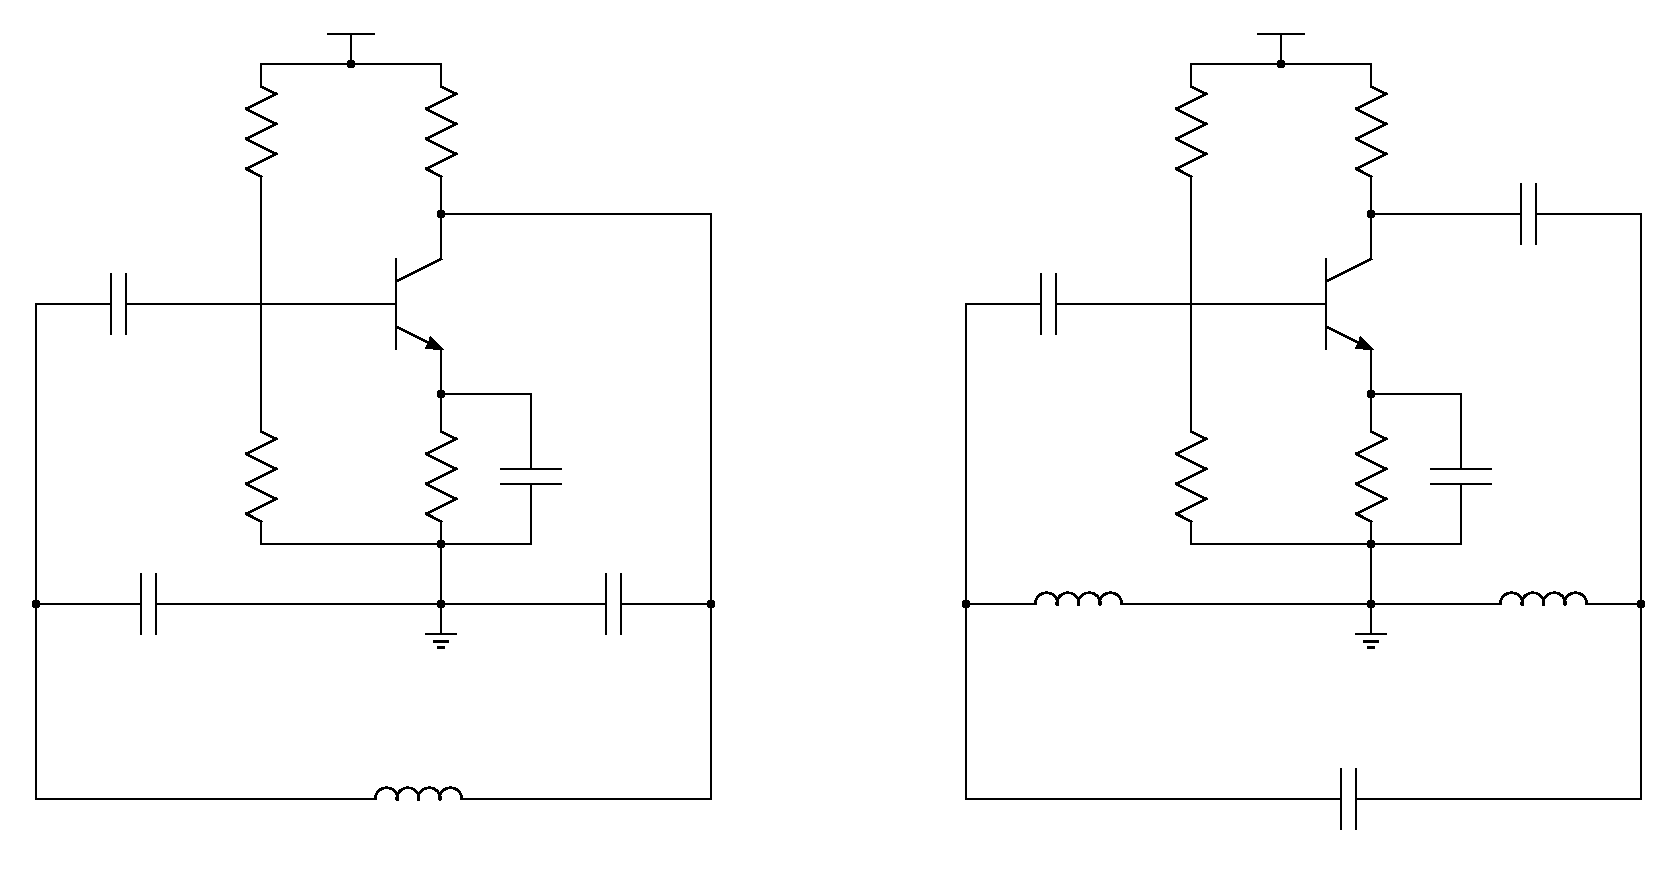
\includegraphics[scale=0.90]{hartleyColpittsOscillator}
\caption{ٹرانزسٹر پر مبنی ہارٹلے اور کالپٹس مرتعش}
\label{شکل_مرتعش_ہارٹلے_کالپٹس}
\end{figure}

شکل \حوالہ{شکل_عمومی_مرتعش} کے عمومی مرتعش میں بنیادی ایمپلیفائر کا داخلی مزاحمت لامحدود ہے جبکہ شکل \حوالہ{شکل_مرتعش_ہارٹلے_کالپٹس} کے دونوں مرتعش میں ایسا نہیں ہے۔

%=====================
\ابتدا{مثال}
ٹرانزسٹر کا پست تعددی ریاضی نمونہ استعمال کرتے ہوئے شکل \حوالہ{شکل_مرتعش_ہارٹلے_کالپٹس} الف کو حل کریں۔حل کرتے وقت بنیادی ایمپلیفائر کے داخلی مزاحمت کو لامحدود تصور کرتے ہوئے نظر انداز کریں۔

حل:شکل \حوالہ{شکل_مرتعش_ہارٹلے_مساوی_پست_تعدد_داخلی_مزاحمت_لامحدود} الف میں اس کا باریک اشاراتی مساوی دور دکھایا گیا ہے جس میں \عددیء{R_1 \mathbin{\|} R_2} کو \عددیء{R_b} لکھا گیا ہے۔بنیادی ایمپلیفائر کا داخلی مزاحمت \عددیء{R_b \mathbin{\|} r_{be}}  کے برابر ہے جو \عددیء{j \omega L_1} کے متوازی جڑا ہے۔\عددیء{\abs{j \omega L_1} \gg R_b \mathbin{\|} r_{be}} تصور کرتے ہوئے  شکل  ب حاصل ہوتا ہے۔
\begin{figure}
\centering
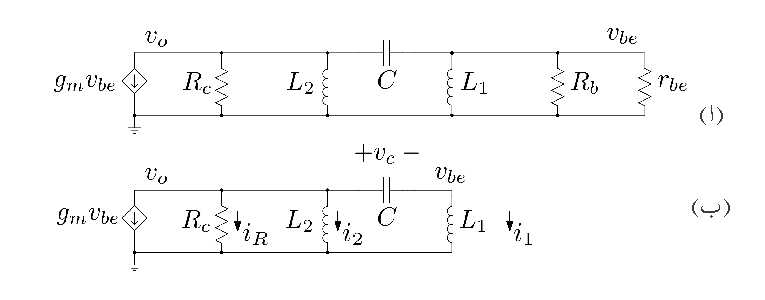
\includegraphics[scale=0.90]{hartleyResistorLoadedEquivalent}
\caption{ٹرانزسٹر پر مبنی ہارٹلے مرتعش کا پست تعددی مساوی دور}
\label{شکل_مرتعش_ہارٹلے_مساوی_پست_تعدد_داخلی_مزاحمت_لامحدود}
\end{figure}

شکل  ب میں اگر ٹرانزسٹر کا داخلی برقی دباو \عددیء{v_{be}} ہو تب \عددیء{L_1} میں برقی رو
\begin{align*}
i_1=\frac{v_{be}}{j \omega L_1}
\end{align*}
ہو گی جو کپیسٹر \عددیء{C} سے گزرتے ہوئے اس پر
\begin{align*}
v_c =\frac{v_{be}}{j \omega L_1} \times \frac{1}{j \omega C}=-\frac{v_{be}}{\omega^2 L_1 C}
\end{align*}
برقی دباو پیدا کرے گا۔یوں
\begin{align*}
v_o&=v_{be}+v_c\\
&=v_{be}-\frac{v_{be}}{\omega^2 L_1 C}
\end{align*}
ہو گا۔\عددیء{L_2} میں
\begin{align*}
i_2&=\frac{v_o}{j \omega L_2}=\frac{v_{be}-\frac{v_{be}}{\omega^2 L_1 C}}{j \omega L_2}
\end{align*}
اور \عددیء{R_c} میں
\begin{align*}
i_R&=\frac{v_o}{R_c}=\frac{v_{be}-\frac{v_{be}}{\omega^2 L_1 C}}{R_c}
\end{align*}
پایا جائے گا۔یوں کرخوف کے قانون برائے برقی رو کی مدد سے ہم لکھ سکتے ہیں
\begin{align*}
-g_m v_{be}&=\frac{v_{be}-\frac{v_{be}}{\omega^2 L_1 C}}{R_c}+\frac{v_{be}-\frac{v_{be}}{\omega^2 L_1 C}}{j \omega L_2}+\frac{v_{be}}{j \omega L_1}\\
&=v_{be} \left[\frac{1}{R_c}-\frac{1}{\omega^2 R_c L_1 C} +\frac{1}{j \omega L_2}-\frac{1}{j \omega^3 L_1 L_2 C} +\frac{1}{j \omega L_1}\right]
\end{align*}
اس مساوات کے خیالی اور حقیقی اور اجزاء علیحدہ علیحدہ کرتے ملتا ہے
\begin{align*}
0&=\frac{1}{j \omega L_2}-\frac{1}{j \omega^3 L_1 L_2 C}+\frac{1}{j \omega L_1} & \textrm{خیالی}\\
-g_m&=\frac{1}{R_c}-\frac{1}{\omega^2 R_c L_1 C} & \textrm{حقیقی}
\end{align*}
خیالی جزو سے
\begin{align}
\omega_0&=\frac{1}{\sqrt{\left(L_1+L_2 \right) C}}
\end{align}
اور حقیقی جزو سے
\begin{align}
g_m R_c=\abs{A_v}=\frac{L_2}{L_1}
\end{align}
حاصل ہوتا ہے۔ان دو مساوات کا مساوات  \حوالہ{مساوات_مرتعش_ہارٹلے_قدرتی_تعدد} اور مساوات \حوالہ{مساوات_مرتعش_عمومی_افزائش} سے موازنہ کریں۔

\انتہا{مثال}
%====================
\ابتدا{مثال}
شکل \حوالہ{شکل_مرتعش_کالپٹس} الف میں ٹرانزسٹر پر مبنی کالپٹس مرتعش دکھایا گیا ہے جس میں ٹرانزسٹر کے کلکٹر پر امالہ \عددیء{L_{\infty}} نسب کیا گیا ہے۔اس امالہ کی قیمت مرتعش کے تعدد پر لامحدود تصور کی جاتی ہے۔مرتعش کو حل کریں۔

حل:شکل  ب میں ٹرانزسٹر کا بلند تعدد ریاضی نمونہ استعمال کرتے ہوئے مرتعش کا مساوی دور دکھایا گیا ہے جہاں مسئلہ ملر کی مدد سے \عددیء{C_{bc}} کا مساوی \عددیء{C_M} دکھایا گیا ہے۔متوازی جڑے مزاحمت \عددیء{R_1}، \عددیء{R_2} اور \عددیء{r_{be}} کو \عددیء{R_m} جبکہ متوازی جڑے کپیسٹر \عددیء{C_{be}}، \عددیء{C_{M}} اور \عددیء{C_1} کو \عددیء{C_1'} لکھتے ہوئے شکل  پ حاصل کی گئی ہے۔حقیقت میں \عددیء{r_{be}} کی قیمت\عددیء{R_1} اور \عددیء{R_2} سے بہت کم ہوتی ہے اور \عددیء{R_m \approx r_{be}} لیا جا سکتا ہے۔  
\begin{figure}
\centering
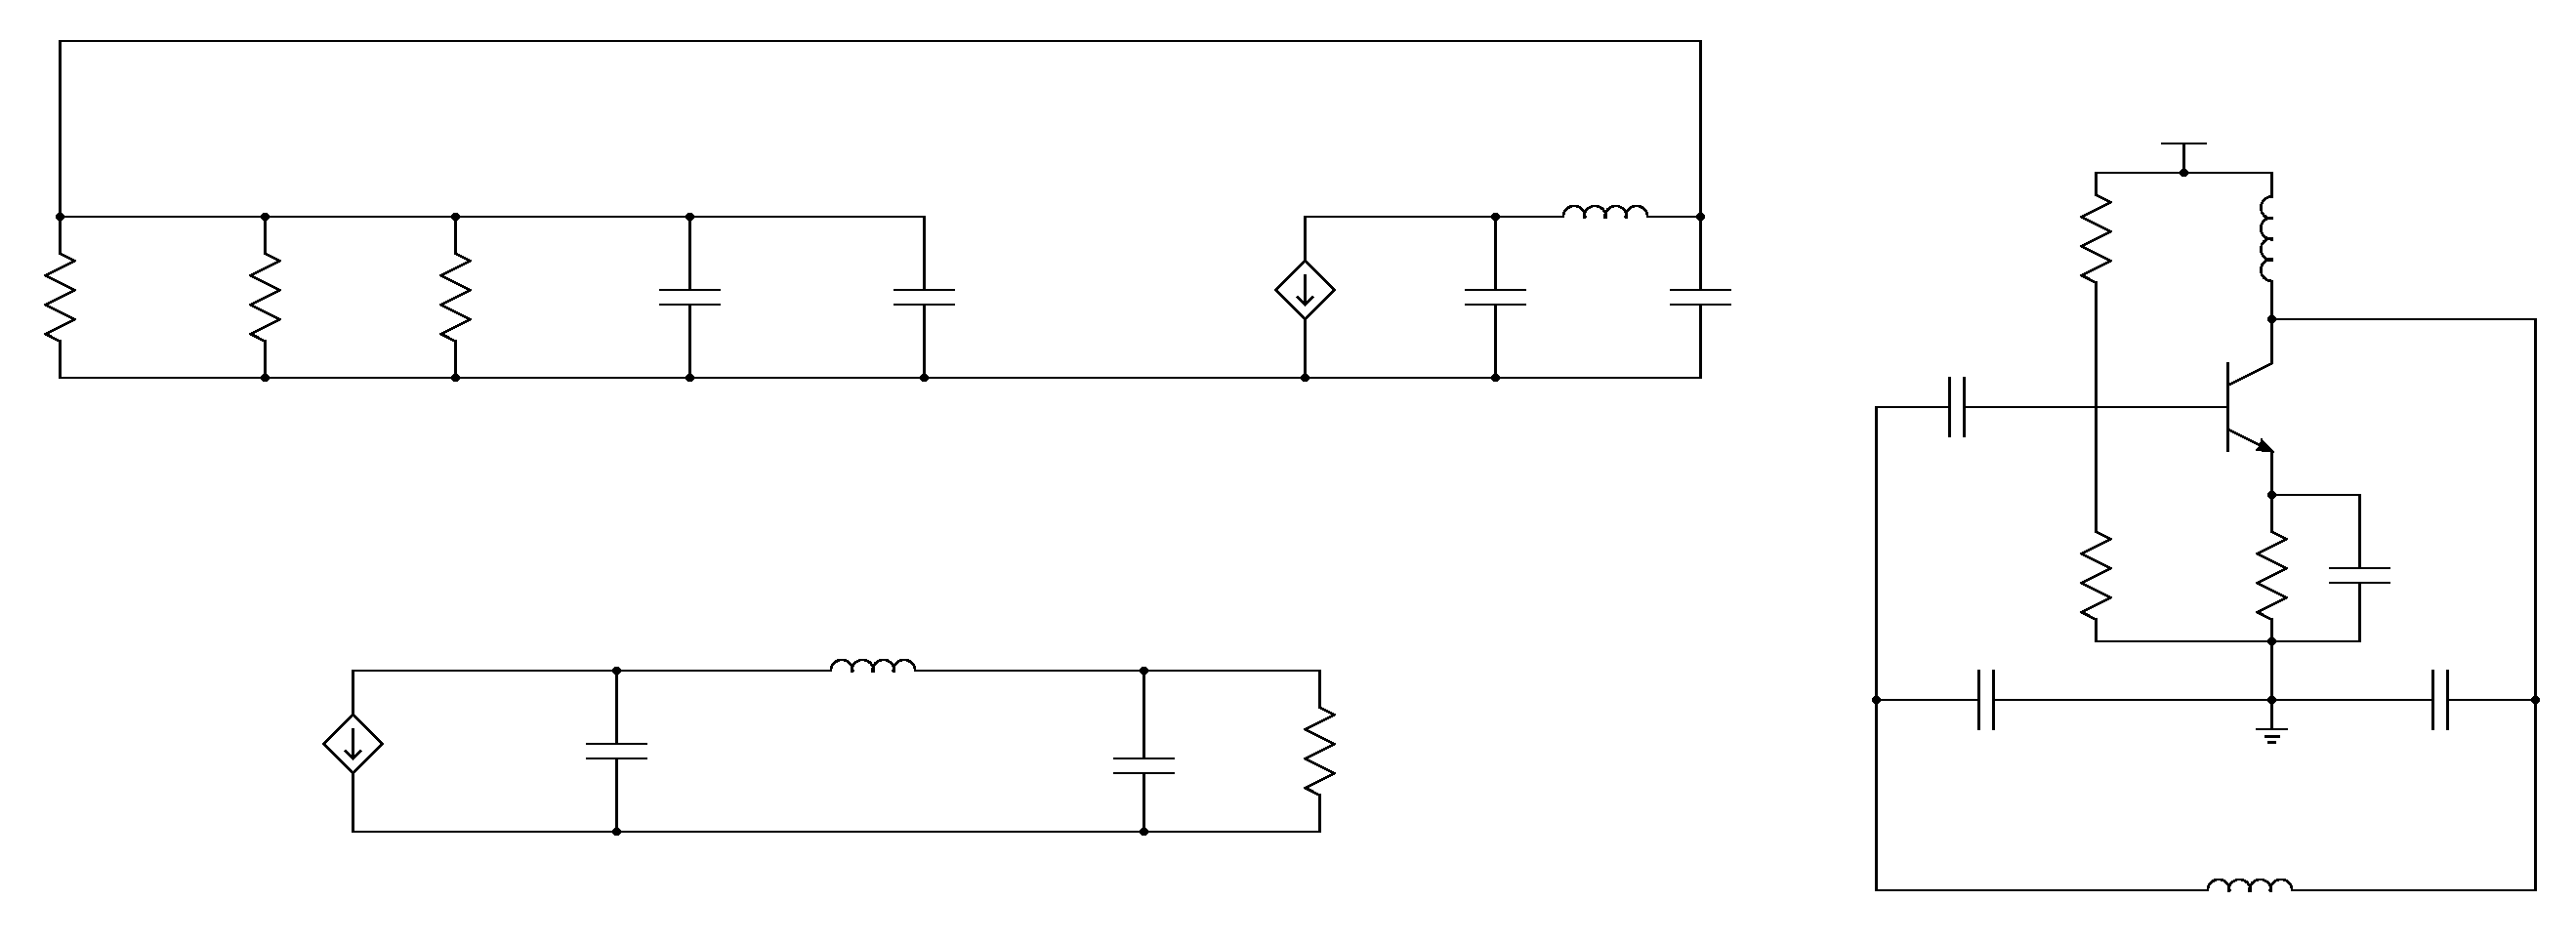
\includegraphics[scale=0.90]{colpittsRadioFreqOscillator}
\caption{ٹرانزسٹر پر مبنی کالپٹس مرتعش}
\label{شکل_مرتعش_کالپٹس}
\end{figure}
\عددیء{R_m} اور \عددیء{C_1'} متوازی جڑے ہیں اور ان پر برقی دباو \عددیء{v_{be}} پایا جاتا ہے۔یوں ان میں برقی رو
\begin{align*}
i_{R_m}&=\frac{v_{be}}{R_m}\\
i_{C_1'}&=j \omega C_1' v_{be}
\end{align*}
ہو گی۔یوں کرخوف کے قانون برائے برقی رو کے تحت
\begin{align*}
i_L=i_{R_m}+i_{C_1'}=\frac{v_{be}}{R_m}+j \omega C_1' v_{be}
\end{align*}
ہو گا۔اس طرح
\begin{align*}
v_L=j \omega L i_L=j \omega L \left(\frac{1}{R_m}+j \omega C_1' \right) v_{be}
\end{align*}
جبکہ
\begin{align*}
v_o&=v_{be}+v_L=\left[1+ j \omega L \left(\frac{1}{R_m}+j \omega C_1' \right) \right] v_{be}
\end{align*}
اور
\begin{align*}
i_{C_2}&=j \omega C_2 v_o=j \omega C_2 \left[1+ j \omega L \left(\frac{1}{R_m}+j \omega C_1' \right) \right] v_{be}
\end{align*}
ہوں گے۔کرخوف کے قانون برائے برقی رو کے تحت \عددیء{i_{C_2}+i_L=-g_m v_{be}} ہے یعنی
\begin{gather}
\begin{aligned} \label{مساوات_مرتعش_ٹرانزسٹر_کالپٹس_مثال_الف}
-g_m v_{be}&=j \omega C_2 \left[1+ j \omega L \left(\frac{1}{R_m}+j \omega C_1' \right) \right] v_{be}+\left(\frac{1}{R_m}+j \omega C_1'\right) v_{be}\\
-g_m&=j \omega C_2 \left[1+ j \omega L \left(\frac{1}{R_m}+j \omega C_1' \right) \right] +\left(\frac{1}{R_m}+j \omega C_1'\right)\\
-g_m&=j \omega C_2 - \omega^2 L C_2 \left(\frac{1}{R_m}+j \omega C_1' \right)  +\frac{1}{R_m}+j \omega C_1'\\
-g_m&=j \omega C_2 -\frac{ \omega^2 L C_2 }{R_m}-j \omega^3 C_1' L C_2  +\frac{1}{R_m}+j \omega C_1'
\end{aligned}
\end{gather}
اس مساوات کے خیالی جزو سے حاصل ہوتا ہے
\begin{align*}
\omega C_2-\omega^3 C_1' L C_2 +\omega C_1' &=0\\
\omega \left(C_2-\omega^2 C_1' L C_2 + C_1'  \right )&=0
\end{align*}
چونکہ چالو مرتعش کی تعدد صفر نہیں ہوتی (یعنی \عددیء{\omega \ne 0}) لہٰذا
\begin{align*}
C_2-\omega^2 C_1' L C_2 + C_1'=0
\end{align*}
ہو گا جس سے حاصل ہوتا ہے
\begin{align}  \label{مساوات_مرتعش_ٹرانزسٹر_کالپٹس_تعدد}
\omega=\omega_o=\sqrt{\frac{C_1'+C_2}{L C_1' C_2}} =\frac{1}{\sqrt{LC}}
\end{align}
جہاں
\begin{align}
\frac{1}{C}=\frac{1}{C_1'}+\frac{1}{C_2}=\frac{C_1'+C_2}{C_1' C_2} 
\end{align}
کے برابر ہے۔\عددیء{\omega_o} مرتعش کی قدرتی تعدد ہے۔

مساوات \حوالہ{مساوات_مرتعش_ٹرانزسٹر_کالپٹس_مثال_الف} کے حقیقی جزو سے حاصل ہوتا ہے۔
\begin{align*}
-g_m&=-\frac{\omega^2 L C_2}{R_m}+\frac{1}{R_m}
\end{align*}
اس میں \عددیء{\omega_o} کی قیمت استعمال کرتے حاصل ہوتا ہے
\begin{align*}
-g_m&=-\left(\frac{C_1'+C_2}{L C_1' C_2} \right)\frac{L C_2}{R_m}+\frac{1}{R_m}\\
g_m R_m&=\frac{C_2}{C_1'}
\end{align*}
\عددیء{R_m \approx r_{be}} لیتے ہوئے اور \عددیء{g_m r_{be}=\beta} کے برابر ہو گا اور یوں مندرجہ بالا مساوات سے حاصل ہو گا
\begin{align} \label{مساوات_مرتعش_ٹرانزسٹر_افزائش}
\beta \approx \frac{C_2}{C_1'}
\end{align}
حقیقت میں \عددیء{\beta} کی قیمت اس مساوات میں دیے قیمت سے زیادہ رکھی جائے گی۔
\انتہا{مثال}

\جزوحصہ{قلمی مرتعش}
ایسا قلم\حاشیہب{crystal} جسے دبانے سے اس کے دو اطراف کے مابین برقی دباو پیدا ہوتا ہے کو \اصطلاح{داب برقی قلم}\فرہنگ{داب برقی قلم}\فرہنگ{piezoelectric crystal}\حاشیہب{piezoelectric crystal} کہتے ہیں۔ \اصطلاح{داب برقی قلم} پر برقی دباو لاگو کرنے سے یہ پھیلتا (یا سکڑتا) ہے۔ایسے \اصطلاح{داب برقی  قلم}  کے قدرتی میکانی تعدد پر برقی دباو فراہم کرتے ہوئے اسے ارتعاش پذیر بنایا جا سکتا ہے۔قلموں کی طبیعیاتی خوبیاں انتہائی مستحکم ہوتی ہیں جو وقت یا حرارت سے بہت کم متاثر ہوتی ہیں۔اسی لئے ایسے قلم کی قدرتی تعدد کی قیمت بھی مستحکم  رہتے ہوئے تبدیل نہیں ہوتی۔اسی خوبی کی بنا پر انہیں عموماً وقت ناپنے کے لئے استعمال کیا جاتا ہے۔\اصطلاح{کوارٹز}\فرہنگ{کوارٹز}\فرہنگ{quartz}\حاشیہب{quartz} گھڑی کا صحیح وقت دکھانا مثالی ہے۔دھاتی ڈبے میں بند، چند کلو ہرٹز \عددیء{\si{\kilo \hertz}} سے کئی میگا ہرٹز \عددیء{\si{\mega \hertz}} تک کے قدرتی تعدد والے کوارٹز کے قلم، منڈی میں عام دستیاب ہیں۔ڈبے پر قلم کی قدرتی تعدد کی قیمت لکھی گئی ہوتی ہے۔
  
\begin{figure}
\centering
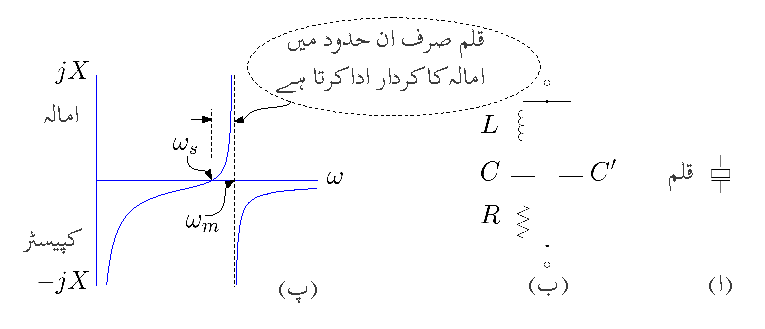
\includegraphics[scale=0.90]{crystalModelAndSymbol}
\caption{داب برقی قلم}
\label{شکل_مرتعش_داب_برقی_قلم}
\end{figure}
%
شکل \حوالہ{شکل_مرتعش_داب_برقی_قلم} الف میں قلم کی علامت دکھائی گئی ہے جبکہ شکل  ب میں اس کا مساوی دور دکھایا گیا ہے۔مساوی دور میں قلم کے میکانی خوبی ماس \عددیء{m} کو امالہ \عددیء{L}، اسپرنگ کے مستقل \عددیء{K} کے معکوس کو کپیسٹر \عددیء{C} اور میکانی مزاحمت کو برقی مزاحمت \عددیء{R} سے  ظاہر کیا جاتا ہے جبکہ \عددیء{C'} قلم کے دونوں سروں پر دھاتی جوڑوں کے مابین کپیسٹر ہے۔

شکل  ب میں مزاحمت \عددیء{R} کو نظرانداز کرتے ہوئے قلم کی برقی رکاوٹ حاصل کرتے ہیں۔
\begin{gather}
\begin{aligned} \label{مساوات_مرتعش_کرسٹل_رکاوٹ_حصول}
\frac{1}{Z}&=j \omega C'+\frac{1}{j \omega L +\frac{1}{j \omega C}}\\
&=\frac{j \omega C' \left( j \omega L +\frac{1}{j \omega C} \right)+1}{j \omega L +\frac{1}{j \omega C}}\\
&=\frac{j \omega C'  \left( j \omega L +\frac{1}{j \omega C} +\frac{1}{j\omega C'}\right)}{j \omega L +\frac{1}{j \omega C}}\\
&=\frac{j \omega C'  \left( j \omega L +\frac{1}{j \omega} \left( \frac{1}{C}+\frac{1}{C'}\right)\right)}{j \omega L +\frac{1}{j \omega C}}
\end{aligned}
\end{gather}
شکل  ب میں  \عددیء{C} اور \عددیء{C'} کو سلسلہ وار جڑے تصور کرتے ہوئے ہم دیکھتے ہیں کہ یہ دونوں \عددیء{L} کے متوازی جڑے ہیں۔یوں \عددیء{L} کے متوازی  جڑے کپیسٹر کو \عددیء{C_m} لکھا جا سکتا ہے جہاں
\begin{align*}
\frac{1}{C_m}=\frac{1}{C}+\frac{1}{C'}
\end{align*}
کے برابر ہے۔اس طرح مساوات \حوالہ{مساوات_مرتعش_کرسٹل_رکاوٹ_حصول} کو یوں لکھا جا سکتا ہے
\begin{align*}
\frac{1}{Z}&=\frac{j \omega C'  \left( j \omega L +\frac{1}{j \omega C_m} \right)}{j \omega L +\frac{1}{j \omega C}}\\
&=\frac{j \omega C'  \left( j \omega L -\frac{j}{\omega C_m} \right)}{j \omega L -\frac{j}{ \omega C}}\\
&=\frac{j \omega C'  \left(\frac{j L}{\omega} \right)\left(\omega^2 -\frac{1}{LC_m} \right)}{ \left(\frac{j L}{\omega} \right) \left(\omega^2 -\frac{1}{LC} \right)}\\
&=\frac{j \omega C'  \left(\omega^2 -\frac{1}{LC_m} \right)}{\left(\omega^2 -\frac{1}{LC} \right)}
\end{align*}
جہاں \عددیء{\frac{1}{j}=-j}  کا استعمال کیا گیا ہے۔

قلم کے دو سروں سے دیکھتے ہوئے \عددیء{L} کے ساتھ \عددیء{C} سلسلہ وار جڑا معلوم ہوتا ہے جبکہ \عددیء{L} کے دو سروں سے دیکھتے ہوئے \عددیء{L} کے ساتھ \عددیء{C_m} متوازی جڑا معلوم ہوتا ہے۔\عددیء{\omega_s^2=\frac{1}{LC}} کو \عددیء{L} اور اس کے ساتھ سلسلہ وار جڑے کپیسٹر \عددیء{C} کی سلسلہ وار قدرتی تعدد جبکہ \عددیء{\omega_m^2=\frac{1}{LC_m}}  کو \عددیء{L} اور اس کے ساتھ متوازی جڑے کپیسٹر \عددیء{C_m} کی متوازی قدرتی تعدد تصور کرتے ہوئے مندرجہ بالا مساوات کو یوں لکھا جا سکتا ہے
\begin{align*}
\frac{1}{Z}&=\frac{j \omega C'  \left(\omega^2 -\omega_m^2 \right)}{\left(\omega^2 -\omega_s^2 \right)}
\end{align*}
جس سے حاصل ہوتا ہے
\begin{align} \label{مساوات_مرتعش_قلم_رکاوٹ}
Z=\frac{-j \left(\omega^2 -\omega_s^2 \right)}{\omega C'  \left(\omega^2 -\omega_m^2 \right)}
\end{align}
اس مساوات کو شکل \حوالہ{شکل_مرتعش_داب_برقی_قلم} پ میں گراف کیا گیا ہے۔حقیقت میں \عددیء{C'} کی قیمت \عددیء{C} کے قیمت سے کئی درجے زیادہ ہوتی ہے (یعنی \عددیء{C' \gg C})۔یوں \عددیء{C_m} کی قیمت \عددیء{C} سے قدر کم  ہوتا ہے جس سے \عددیء{\omega_s} کی قیمت \عددیء{\omega_m} کے قیمت سے قدر کم ہوتا ہے۔ان دو قدرتی تعدد کی قیمتوں میں \عددیء{1 \%} سے بھی کم فرق ہوتا ہے۔مساوات \حوالہ{مساوات_مرتعش_قلم_رکاوٹ} میں دیا برقی رکاوٹ \عددیء{\omega_s < \omega < \omega_m} کے حدود میں بطور امالہ جبکہ \عددیء{\omega< \omega_s} یا \عددیء{\omega>\omega_m} کے حدود میں بطور کپیسٹر  کردار ادا کرتا ہے۔

مندرجہ بالا تذکرے کو مدِ نظر رکھتے ہوئے ہم دیکھتے ہیں کہ کالپٹس مرتعش میں امالہ کی جگہ قلم استعمال کیا جا سکتا ہے۔شکل \حوالہ{شکل_مرتعش_کالپٹس} میں ایسا کرتے ہوئے  شکل \حوالہ{شکل_کالپٹس_ہارٹلے_مرتعش_قلمی} الف کا \اصطلاح{کالپٹس قلمی مرتعش} حاصل ہوتا ہے۔چونکہ قلم صرف \عددیء{\omega_s < \omega < \omega_m} حدود میں بطور امالہ کردار ادا کرتا ہے لہٰذا ایسا مرتعش صرف اور صرف انہیں حدود کے درمیان ارتعاش پذیر رہ سکتا ہے اور اس کی تعدد انہیں حدود کے درمیان رہے گی۔آپ دیکھ سکتے ہیں کہ \اصطلاح{قلمی مرتعش}\فرہنگ{قلمی مرتعش}\فرہنگ{مرتعش!قلمی}\فرہنگ{crystal oscillator}\حاشیہب{crystal oscillator} کی تعدد صرف اور صرف قلم کی قدرتی تعدد پر منحصر ہے۔اب چونکہ \عددیء{\omega_s \approx \omega_m} ہوتا ہے لہٰذا حقیقت میں ایسے مرتعش کی  \عددیء{\omega \approx \omega_s \approx \omega_m} رہے گی۔چونکہ مساوات \حوالہ{مساوات_مرتعش_ٹرانزسٹر_کالپٹس_تعدد} بھی اس مرتعش کی تعدد دیتا ہے لہٰذا قلمی مرتعش اپنی تعدد \عددیء{\omega_s} اور \عددیء{\omega_m} کے درمیان اس جگہ برقرار رکھے گا جہاں مساوات \حوالہ{مساوات_مرتعش_قلم_رکاوٹ} سے حاصل قلم کی  برقی رکاوٹ (یعنی \عددیء{L}) کو استعمال کرتے ہوئے مساوات \حوالہ{مساوات_مرتعش_ٹرانزسٹر_کالپٹس_تعدد} سے بھی یہی تعدد حاصل ہو۔قلمی مرتعش کے استعمال کا مقصد ایک حتمی تعدد حاصل کرنا ہے جو قلم کو \عددیء{\omega_s \approx \omega_m} حدود میں استعمال کرتے حاصل ہوتا ہے ۔

شکل \حوالہ{شکل_کالپٹس_ہارٹلے_مرتعش_قلمی} ب میں قلمی ہارٹلے مرتعش دکھایا گیا ہے۔\عددیء{C'} کو نظرانداز کرتے اور قلم کو امالہ تصور کرتے ہوئے  \عددیء{L}، \عددیء{C} اور قلم  ہارٹلے مرتعش کی جانی پہچانی شکل میں جڑے ہیں۔\عددیء{C'} کی قیمت اتنی رکھی جاتی ہے کہ درکار تعدد پر متوازی جڑے \عددیء{L} اور \عددیء{C'} (جنہیں عام فہم میں \عددیء{LC} \اصطلاح{ٹینک}\فرہنگ{ٹینک}\فرہنگ{مرتعش!ٹینک}\فرہنگ{tank}\حاشیہب{tank} کہا جاتا ہے) کا مجموعہ امالہ کا کردار ادا کرے۔عموماً \عددیء{C'} قابل تبدیل کپیسٹر ہوتا ہے جس کی قیمت تبدیل کرتے ہوئے  مرتعش کی تعدد باریکی سے قابو کی جاتی ہے۔چونکہ متوازی جڑے \عددیء{LC} کی برقی رکاوٹ ان کے قدرتی متوازی تعدد پر لامحدود ہوتی ہے لہٰذا \عددیء{LC} ٹینک کی قدرتی متوازی تعدد کو مرتعش کے تعدد کے قریب رکھتے ہوئے  \عددیء{nJFET} کے ڈرین پر بہت زیادہ برقی رکاوٹ حاصل کیا جاتا ہے جس سے  بنیادی ایمپلیفائر کی افزائش زیادہ حاصل ہوتی ہے اور ارتعاشی اشارے کا حیطہ زیادہ سے زیادہ حاصل کرنا ممکن ہوتا ہے۔اس مرتعش میں بیرونی کپیسٹر \عددیء{C} کا استعمال ضروری نہیں۔نہایت بلند تعدد حاصل کرتے وقت اس کپیسٹر کو نسب نہیں کیا جاتا اور \عددیء{nJFET} کی اندرونی کپیسٹر \عددیء{C_{gd}} اور \عددیء{nJFET} کے ڈرین اور گیٹ کے مابین تاروں کے  مابین  بلا ارادہ پائے جانے والے کپیسٹر کو زیر استعمال لایا جاتا ہے۔
\begin{figure}
\centering
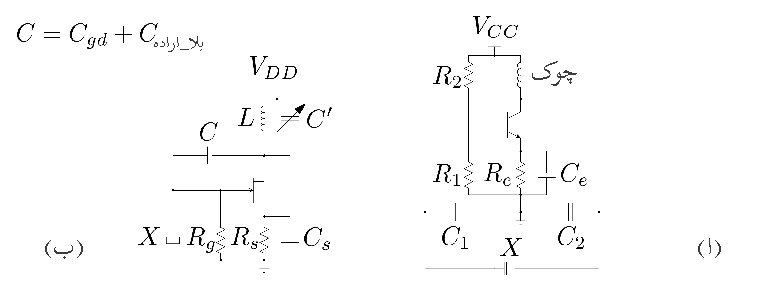
\includegraphics[scale=0.90]{crystalColpittsHartleyOscillator}
\caption{قلمی کالپٹس اور ہارٹلے مرتعش}
\label{شکل_کالپٹس_ہارٹلے_مرتعش_قلمی}
\end{figure}
%====================
\newpage
\حصہء{سوالات}

\ابتدا{سوال}\شناخت{سوال_مرتعش_مزاحمت_کپیسٹر_دو_کڑی}
شکل \حوالہ{شکل_مزاحمت_کپیسٹر_زاویہ_میں_تبدیلی} ب میں \عددیء{RC} کے دو حصے ترتیب وار جوڑے گئے ہیں۔اس میں \عددیء{\frac{\hat{V_o}}{\hat{V_i}}}  کی مساوات حاصل کریں۔اگر \عددیء{f=\SI{10}{\kilo \hertz}}  اور \عددیء{C=\SI{0.01}{\micro \farad}} ہوں تب \عددیء{\hat{V_o}} اور \عددیء{\hat{V_i}} میں کل \عددیء{\SI{-120}{\degree}} کا زاویہ حاصل کرنے کی خاطر درکار مزاحمت حاصل کریں۔

جوابات:
\begin{align*}
\frac{\hat{V_o}}{\hat{V_i}}&=\frac{1}{1+j 3 \omega R C -\omega^2 R^2 C^2}\\
R&=\SI{1196}{\ohm}
\end{align*}
\انتہا{سوال}
%==================
\ابتدا{سوال}
\عددیء{RC} مرتعش میں کم سے کم ممکنہ \عددیء{\beta} کا ٹرانزسٹر استعمال کیا جاتا ہے۔\عددیء{R=\SI{200}{\ohm}} کی صورت میں \عددیء{Z_{RC}} کی قیمت حاصل کریں۔

جواب:\عددیء{Z_{RC}=372-j 198}
\انتہا{سوال}
%==================
\ابتدا{سوال}
شکل \حوالہ{شکل_مزاحمت_کپیسٹر_مرتعش} میں \عددیء{RC} مرتعش دکھایا گیا ہے جس میں
\begin{align*}
V_{CC}&=\SI{9}{\volt}, \hspace{5mm} R_c=\SI{3}{\kilo \ohm}, \hspace{5mm} R_e=\SI{1}{\kilo \ohm}\\
R_1&=\SI{12.5}{\kilo \ohm}, \hspace{5mm} R_2=\SI{50}{\kilo \ohm}, \hspace{5mm} \beta=99
\end{align*}
ہیں۔\عددیء{\SI{10}{\kilo \hertz}} پر چلنے کی خاطر درکار \عددیء{C} اور \عددیء{R'} حاصل کریں۔

جوابات:\عددیء{I_{CQ}=\SI{1}{\milli \ampere}} اور \عددیء{r_{be}=\SI{2.54}{\kilo \ohm}} ہیں۔\عددیء{k=2.69} استعمال کرتے ہوئے \عددیء{R=\SI{1115}{\ohm}}حاصل ہوتا ہے جس سے \عددیء{C=\SI{3.5}{\nano \farad}} حاصل ہوتا ہے۔\عددیء{R_m=\SI{2}{\kilo \ohm}} حاصل ہوتا ہے۔چونکہ \عددیء{R_m > R'} ہے لہٰذا تمام \عددیء{R} برابر رکھنا ممکن نہ ہو گا اور یوں \عددیء{R'=\SI{0}{\ohm}} رکھا جائے گا۔قدرتی تعدد \عددیء{\SI{10}{\kilo \hertz}} سے قدر مختلف ہو گی۔
\انتہا{سوال}
%==================
\ابتدا{سوال}
شکل \حوالہ{شکل_مزاحمت_کپیسٹر_مرتعش} کے \عددیء{RC} مرتعش میں
\begin{align*}
V_{CC}&=\SI{9}{\volt}, \hspace{5mm} R_c=\SI{3.36}{\kilo \ohm}, \hspace{5mm} R_e=\SI{1}{\kilo \ohm}\\
R_1&=\SI{6.25}{\kilo \ohm}, \hspace{5mm} R_2=\SI{25}{\kilo \ohm}, \hspace{5mm} \beta=49
\end{align*}
ہیں۔\عددیء{\SI{10}{\kilo \hertz}} پر چلنے کی خاطر درکار \عددیء{C} اور \عددیء{R'} حاصل کریں۔

جوابات:\عددیء{I_{CQ}=\SI{1}{\milli \ampere}} اور \عددیء{r_{be}=\SI{1.25}{\kilo \ohm}} ہیں۔\عددیء{k=2.69} کی صورت میں \عددیء{R=\SI{1250}{\ohm}} حاصل ہوتا ہے جس سے \عددیء{C=\SI{3.1}{\nano \farad}} حاصل ہوتا ہے۔\عددیء{R_m=\SI{1}{\kilo \ohm}} حاصل ہوتا ہے  یوں \عددیء{R'=\SI{250}{\ohm}} رکھا جائے گا۔
\انتہا{سوال}
%============
\ابتدا{سوال}
صفحہ \حوالہصفحہ{شکل_مرتعش_وائن} پر شکل \حوالہ{شکل_مرتعش_وائن} میں وائن مرتعش دکھایا گیا ہے۔\عددیء{R=\SI{15.9}{\kilo \ohm}}، \عددیء{C=\SI{0.1}{\micro \farad}}، \عددیء{R_1=\SI{10}{\kilo \ohm}} اور \عددیء{R_2=\SI{25}{\kilo \ohm}} کی صورت میں مرتعش کی قدرتی تعدد حاصل کریں۔

جواب:\عددیء{f_o=\SI{100}{\hertz}}
\انتہا{سوال}
%================
\ابتدا{سوال}
شکل \حوالہ{شکل_ٹرانزسٹر_ہمسر_مرتعش} میں ٹرانزسٹر کا \عددیء{\beta=39}، \عددیء{V_A=\SI{200}{\volt}} اور \عددیء{C_{be}=\SI{10}{\pico \farad}} اور \عددیء{C_{bc}=\SI{4}{\pico \farad}} ہیں جبکہ \عددیء{R_B=\SI{5}{\kilo \ohm}} اور \عددیء{I_{CQ}=\SI{1}{\milli \ampere}} ہیں۔ٹرانسفارمر کی \عددیء{\tfrac{n_1}{n_2}} حاصل کریں۔اگر \عددیء{C=\SI{20}{\nano \farad}} اور \عددیء{L=\SI{200}{\nano \henry}} ہوں تب \عددیء{f_o} کیا ہو گا۔

جوابات:\عددیء{\tfrac{n_2}{n_1}=0.02564}، \عددیء{g_m=\SI{0.04}{\siemens}}، \عددیء{r_{be}=\SI{925}{\ohm}}، \عددیء{r_o=\SI{200}{\kilo \ohm}}، \عددیء{R_p'=\SI{0.51}{\ohm}}، \عددیء{R \approx \SI{0.51}{\ohm}}، \عددیء{C_M \approx \SI{4}{\pico \farad}}، \عددیء{C_p=\SI{39.166}{\nano \farad}} ہیں اور یوں \عددیء{f_o=\SI{1.798}{\mega \hertz}} ہو گا۔
\انتہا{سوال}
%================
\ابتدا{سوال}\شناخت{سوال_مرتعش_پست_کالپٹس}
شکل \حوالہ{شکل_مرتعش_ہارٹلے_کالپٹس} ب میں \عددیء{R_c} کی جگہ لامحدود \عددیء{L} نسب کیا جاتا ہے۔\عددیء{R_B} کو نظر انداز کرتے اور ٹرانزسٹر کا پست تعددی مساوی پائے ریاضی نمونہ استعمال کرتے ہوئے اسے حل کریں۔

جوابات:\عددیء{\omega_o=\tfrac{1}{\sqrt{LC}}} جہاں \عددیء{C=\tfrac{C_1 C_2}{C_1+C_2}} کے برابر ہے جبکہ \عددیء{\beta =\tfrac{C_2}{C_1}} حاصل ہوتا ہے۔
\انتہا{سوال}
%================
\ابتدا{سوال}\شناخت{سوال_کالپٹس_مرتعش_پست-تعدد}
سوال \حوالہ{سوال_مرتعش_پست_کالپٹس} کے کالپٹس مرتعش میں ٹرانزسٹر کا \عددیء{\beta=50} ہے۔اگر اس میں \عددیء{C_1=\SI{0.01}{\micro \farad}} رکھا جائے تب \عددیء{\SI{200}{\kilo \hertz}} پر ارتعاش کرتے مرتعش کے بقایا اجزاء کے قیمتیں کیا ہوں گی؟

جوابات:\عددیء{C_2=\SI{0.5}{\micro \farad}}، \عددیء{L=\SI{65}{\micro \farad}}
\انتہا{سوال}
%==============
\ابتدا{سوال}\شناخت{سوال_ہارٹلے_مرتعش_پست_تعدد}
شکل \حوالہ{شکل_مرتعش_ہارٹلے_کالپٹس} کے کالپٹس مرتعش میں ٹرانزسٹر کا پست تعددی ریاضی نمونہ استعمال کرتے ہوئے حل کریں۔ایسا کرتے ہوئے بنیادی ایمپلیفائر کی داخلی مزاحمت  لامحدود تصور کریں۔

جوابات:\عددی{\omega_o=\tfrac{1}{\sqrt{LC}}} جہاں \عددیء{C=\tfrac{C_1 C_2}{C_1+C_2}} کے برابر ہے ، \عددیء{g_m R_c=\tfrac{C_1}{C_2}}۔ ان مساوات کا مساوات \حوالہ{مساوات_مرتعش_عمومی_افزائش} اور مساوات \حوالہ{مساوات_مرتعش_کالپٹس_قدرتی_تعدد} کے ساتھ موازنہ کریں۔
\انتہا{سوال}
%================
